
%!TEX ROOT=DavidPetrDP.tex
\chapter{Realizace FW}
\section{Struktura FW}
Jak vyplývá ze zadání, firmware vznikal v návaznosti na existující přístroj využívající stávající PC aplikací Zero eLab Viewer a již touto skutečností byl návrh firmware mikrokontroléru částečně vymezen. Přestože určité změny PC aplikace by byli přípustné, tak bylo podstatné aby přes jakékoliv provedené změny aplikace zůstala použitelná i pro všechny dříve vzniklé implementace SDI pro jiné mikrokontroléry. Především pak komunikační protokol, který se v některých případech prokázal limitující nemohl být upraven. Dále není jednoduché přidávat funkcionality se kterými původně aplikace nepočítala a tedy aplikace rovnou určuje jaké softwarově definované přístoje lze implementovat a jaké budou mít možnosti ovládání či nastavení. Při návrhu Fw jsem se pak zaměřil na tyto body

\begin{itemize}
	\item \textbf{Samostatná využitelnost jednotlivých přístrojových bloků}\\ 
	Rozdělit implementaci jednotlivých přístrojů do samostatně fungujících bloků je výhodné z 2 důvodů. Zaprvé lze tak jednodušeji výsledný FW přizpůsobit pro různé mikrokontroléry v závislosti na dostupných periferií a velikosti FLASH paměti. Druhým důvodem je možnost použití částí kódu jako příklady pro návrh nově vznikajících SDI přístrojů .
	\item  \textbf{Jednoduchá záměna HW prostředků}\\
	Bylo žádoucí, aby vznikající FW byl flexibilní, co se týče použitých HW prostředků a tedy aby bylo například možné jednoduše upravovat použité piny, DMA kanály či čítače. Toto dále zjednodušuje další adaptaci firmware pro jiné MCU.	
	\item \textbf{Kompaktibilita s generátorem inicializačního kódu}\\	
	Nástroj STM32CubeMX velmi usnadňuje začátek vytváření FW díky využití grafického rozhraní pro definování počáteční konfigurace MCU. Pokud se zachová struktura generovaného kódu, lze pak nástroj opětovně využít v případě, že chceme jednoduše upravit HW konfiguraci.
\end{itemize}


\begin{figure}[H]
	\centering
	
\includegraphics[width=0.9\linewidth]{Figs/Documentation/FW_Zavislosti}
	\caption{Kategorie zdrojového kodu a jejich posloupnost závislosti}
	\label{fig:fwzavislosti}
\end{figure}


\subsection{Využití možnosti přepínání mezi konfiguracemi}
Především z důvodů omezených hardwarových prostředků na různých mikrokontrolérech je využito možnosti přepínání různých přístrojových konfigurací. Konfigurací v tomto případě myslíme set nástrojů, které mohou být použity současně. Přístrojové moduly pak mohou sdílet periferie za předpokladu, že v dané konfiguraci je aktivní pouze jeden z těch modulů, který má přístup k dané periferii. Příkladem může být sdílení ADC převodníku modulem Voltmetru a modulem Osciloskopu, které pak tedy nemohou být aktivní zároveň. Jako je vidět na obrázku \ref{fig:zeroelab} hlavního okna PC aplikace.

\begin{figure}[H]
	\centering
	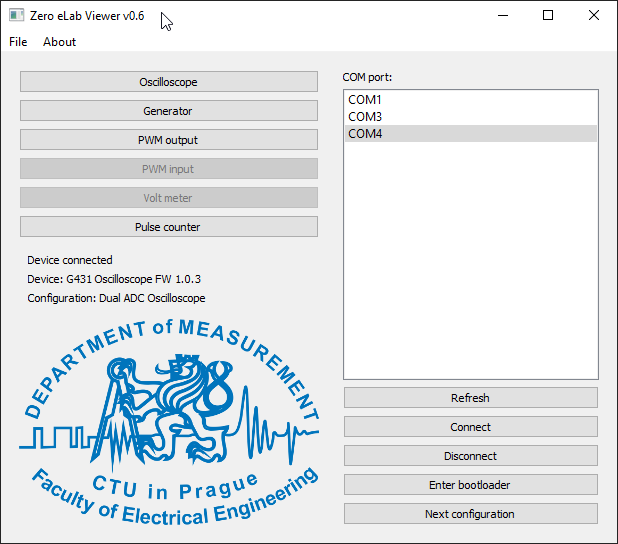
\includegraphics[width=0.7\linewidth]{Figs/Screenshots/ZeroElab}
	\caption{Hlavní okno aplikace Zero eLab Viewer zobrazující aktivní moduly dané konfigurace}
	\label{fig:zeroelab}
\end{figure}

\subsection{Využití LL ovladačů}
Firma STMicroelectronics pro podporu svého portfólia mikrokontrolérů nabízí tzv. LL ovladače usnadňující psaní firmware. Jedná se o hardwarově orientovanou knihovnu jejíž využití je velmi podobné využití CMSIS ovladačů s tím rozdílem, že nabízí určité rozšířené možnosti portovatelnosti mezi jednotlivými rodinami mikrokontrolérů a sadu rozšiřujících API pro zjednodušení implementace některých úkonů, jako je například inicializace periferií. K použití této knihovny je oproti pravděpodobně známější knihovně HAL zapotřebí znalost jednotlivých periferií, jelikož velká část definovaných funkcí je pouze jednořádková modifikace registrů bez kontrol vstupních parametrů a uživatel tedy musí být více obeznámen s tím co dělá. Výhodou LL oproti HAL je výrazně menší délka generovaného kódu a tedy nižší paměťová náročnost.\\

Pro vytvoření představy o rozdílnosti paměťové náročnosti jednotlivých knihoven jsem vytvořil pomocí STM32CubeMX dva minimální projekty, jejichž úkolem bylo pouze inicializace systémových hodin a dále blikání jednou LED. V prvním případě byly periferie RCC(Reset and clock control) a GPIO inicializovány prostřednictvím HAL knihovny a v druhém případě pomocí LL ovladačů a byly použity odpovídají zpožďovací funkce společně s přepínáním výstupu pinu. Výsledkem bylo, že  po zkompilování verze s HAL knihovnou využívala asi o 46 procent více FLASH paměti.

\begin{table}[H]
	\begin{tabular}{l|ll}
		& FLASH   & RAM     \\ \hline
		LL ovlačače                       & 3.04 kB & 1,53 kB \\
		\multicolumn{1}{c|}{HAL ovladače} & 5,66 kB & 1,55 kB
	\end{tabular}
	\caption{Srovnání paměťové náročnosti jednoduchého programu s využitím různých knihoven}
	\label{tab:LL_HAL_MemoryUsage}
\end{table}	

\section{Rozpoznání frekvence externího krystalu HSE}
Pro chod mikrokontroléru je zapotřebí zdroj hodinového signálu pro generování systémových hodin (System Core clock), dále jen SYSCLK. Jako základní varianta zdroje hodinového signálu se používá interní vysoko-rychlostní oscilátor (HSI), jehož výstupní frekvence ve srovnání s externími zdroji hodinového signálu vykazuje řádově vyšší nepřesnost a vyšší závislost na změnách teplot viz srovnávací tabulka \ref{tab:HSE}.Tento rozdíl je pak obzvlášť podstatný při realizaci funkce osciloskopu v režimu vzorkování v ekvivalentním čase (ETS), kde dochází k výraznému zkreslení měřeného signálu viz obrázek \ref{fig:signaldistortionhsi}. Na tomto obrázku je zobrazen zkreslený záznam signálu s G431 využívajícím HSI jako zdroj hodinového signálu a druhá stopa je měřena osciloskopem Rigol DS1052E, jehož přesnost vzorkovací frekvence je $\pm0.005\%$ \cite{ScopeRigol}. Z obrázku je zřejmá vhodnost použití zdroje hodinového signálu s vyšší přesností než vykazuje HSI.

\begin{figure}[H]
	\centering
	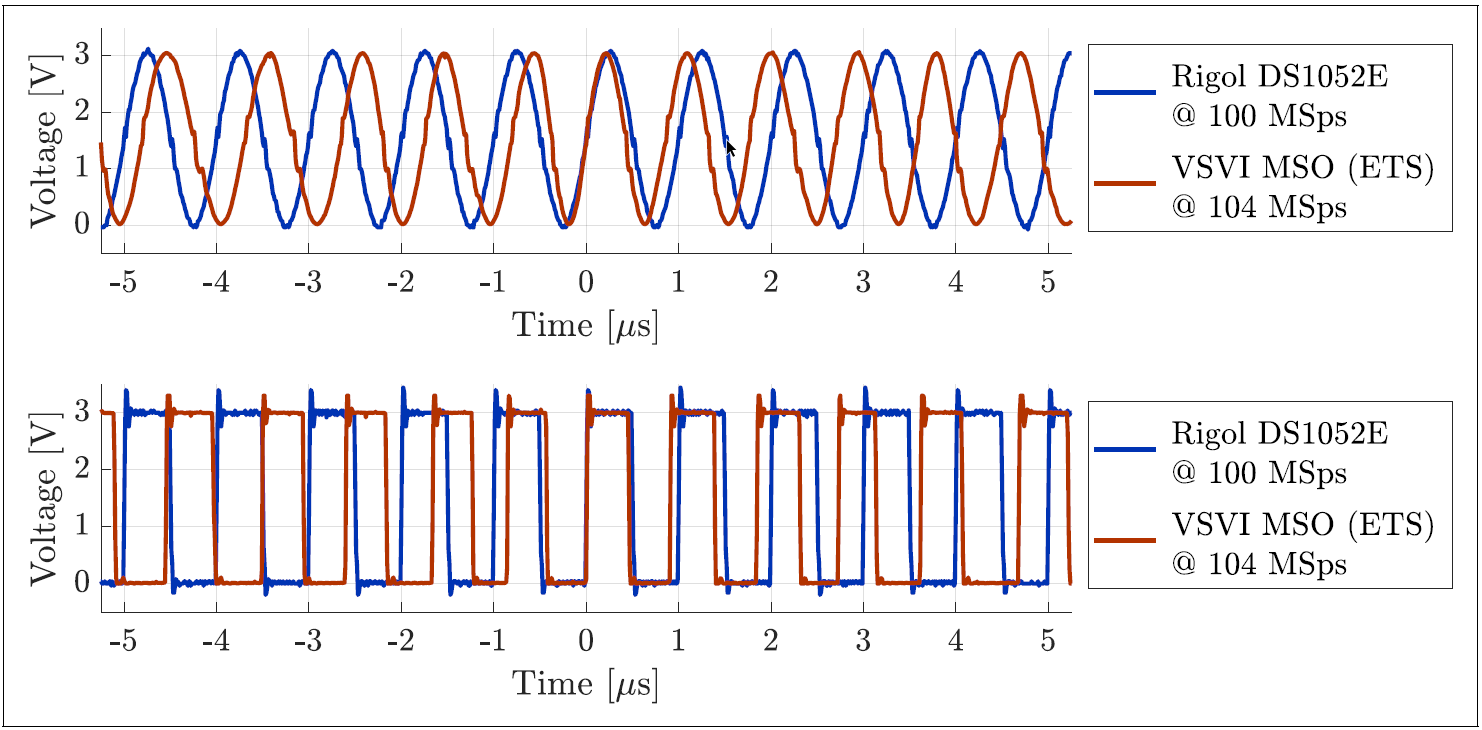
\includegraphics[width=0.7\linewidth]{Figs/Graphs/SignalDistortion_HSI}
	\caption{Zkreslení průběhu měřeného signálu v důsledku nestability HSI převzato z \cite{DujavaDIP}}
	\label{fig:signaldistortionhsi}
\end{figure}

Jako zdroj vysokorychlostního externě získaného hodinové signálu (HSE) lze buď využít krystalu buzeného pomocí MCU (HSE crystal) nebo jiného externího zdroje signálu (HSE bypass) splňující podmínky na maximální frekvenci a střídu hodinového signálu pro dané MCU. Například pro STM32G431 musí být externí signál v rozsahu 4-48MHz a mít střídu 40-60\%. Ve výuce laboratorních měření na katedře měření jsou k dispozici krystaly různých výstupních frekvencí převážně pak 8 MHz, 12MHz a 16MHz. Pro  účely co nejflexibilnějšího laboratorního přístroje se zdálo účelné naprogramovat firmware pro použití s různými  oscilátory tohoto typu. Tedy aby funkce FW nebyla závislá na přítomnosti krystalu ani jeho výstupní frekvenci. Toho bylo docíleno změřením výstupní frekvence oscilátoru a nastavení výsledné frekvence systémových hodin pomocí interního obvodu fázového závěsu(PLL), tak aby výsledná frekvence SYSCLK nebyla na použitém krystalu závislá.


\begin{table}[H]
	\begin{tabular}{l|rr}
		&\multicolumn{1}{c}{\begin{tabular}[c]{@{}c@{}}Absolutní\\ odchylka frekvence\end{tabular}} & \multicolumn{1}{c}{\begin{tabular}[c]{@{}c@{}}Odchylka frekvence \\ způsobená změnou teploty\end{tabular}} \\ \hline
		STM32G431 HSI 16 MHz     & $\pm$ 1\%       & $\pm$1\%    (~~0 až +85$^\circ$C) \\
		Adafruit krystal 16 MHz & $\pm$0.003\%   & $\pm$0.005\%  (-20 až +70$^\circ$C)
	\end{tabular}
	\caption{}
	\label{tab:HSE}
\end{table}

\subsection{Měření frekvence HSE}
\label{ch:HSEFrequencyMeas}
Abychom mohli správně nastavit parametry PLL podle použitého krystalu, potřebujeme znát jeho frekvenci. Variantou by mohlo být ponechat na uživateli, aby zadal použitou frekvenci krystalu například nějakou zprávou přijatou z aplikace v počítači. Nicméně pro to by se musela upravit aplikace. Jako optimálnější řešení se zdálo frekvenci dostupného krystalu změřit. Na rodině mikrokontrolérů STM32G4 mají čítače TIM16 a TIM17 možnost interně přivést HSE se sníženou frekvencí. Frekvence HSE je totiž ještě před přivedením na vstup čítače zpracovaná obvodem, který frekvenci 32krát sníží. Pro tento vstup čítače se sníženou frekvencí se pak používá označení HSE/32 jako je vidět na obrázku \ref{fig:tim16inputs} z dokumentace.

\begin{figure}[H]
	\centering
	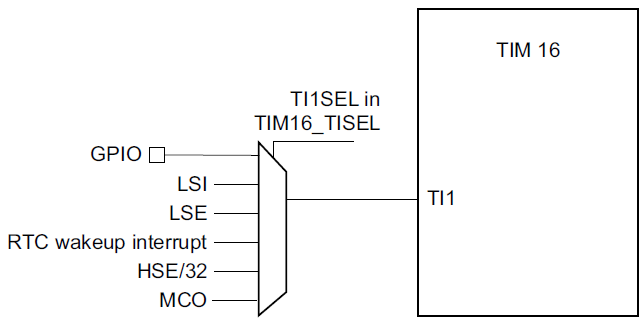
\includegraphics[width=0.7\linewidth]{Figs/Documentation/TIM16_Inputs}
	\caption[Vstupy čítače TIM16]{Vstupy dostupné na kanálu číslo 1 čítače TIM16. Převzato z\cite{refG4}}
	\label{fig:tim16inputs}
\end{figure}

Standardní způsob měření periody vstupního signálu probíhá potom tak, že měříme počet uběhlých cyklů čítače mezi jednotlivými náběžnými hranami nebo sestupnými hranami jako je vyobrazeno na obrázku \ref{fig:PeriodMeasurement}. Tento počet cyklů nám pak určuje poměr mezi frekvencí externího hodinového signálu na vstupu $	f_{\text{IN}}$ a hodinového signálu, který pro svůj chod využívá periferie čítače $	f_{\text{TIM}}$. Druhou zmíněnou frekvenci($f_{\text{TIM}}$) typicky známe. Pro správné měření je také podstatné, aby frekvence interního hodinového signálu čítače byla výrazně vyšší než frekvence na měřeném vstupu. Pro získání přesnějšího odhadu vstupní frekvence můžeme zaznamenat více period po sobě a ty  zprůměrovat. Na obrázku \ref{fig:PeriodMeasurement} je popsán případ, kdy ze záznamu paměti je vidět, že jednotlivé odebrané vzorky jsou od sebe vzdáleny tři periody interních hodin PCLK. Frekvence vstupního signálu $f_{\text{IN}}$ je tedy třetinová oproti frekvenci $f_{\text{TIM}}$
\begin{equation}
	f_{\text{IN}}=\frac{f_{\text{TIM}}}{N_\text{period}}=\frac{f_{\text{TIM}}}{\text{buf[n]}-\text{buf[n-1]}}=\frac{f_{\text{TIM}}}{3}
\end{equation}

V případě měření frekvence HSE o frekvenci $f_{\text{HSE\_8}}=8 \text{MHz}$ přivedený na zmíněný vstup čítače s vestavěnou předděličkou HSE/32 a frekvencí vnitřních hodin $f_{\text{TIM}}=156$ MHz. Tak můžeme  očekávat následující počet period mezi jednotlivými náběžnými hranami:
\begin{equation}
N_\text{period}=\frac{f_{\text{TIM}}}{f_{\text{IN}}},\quad f_{\text{IN}}=\frac{f_{\text{HSE}}}{32} \implies N_\text{HSE\_8}=\frac{32 f_{\text{TIM}}}{f_{\text{HSE\_8}}}= 624
\end{equation}
Obdobně pro krystal s frekvencí $f_{\text{HSE\_16}}=16 \text{ MHz}$ bychom změřili, že mezi jednotlivými náběžnými hranami vstupního signálu uběhne $N_\text{HSE\_16}= 312$ period vnitřních hodin čítače. Tedy vysoká frekvence vnitřních hodin čítače  $f_{\text{TIM}}=156$ MHz a možnost dělení signálu HSE před samotným vstupem do periferie čítače poskytuje dostatečnou rozlišovací schopnost mezi jednotlivými krystaly, abychom je od sebe dokázali rozlišit.
     

\begin{figure}[H]
	\centering
	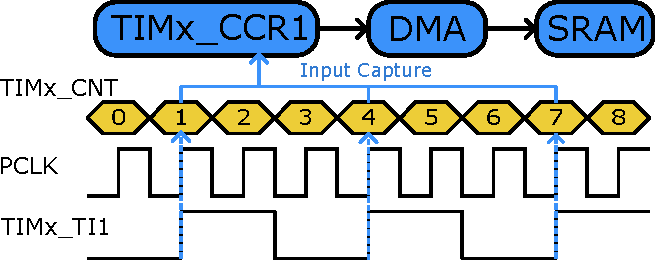
\includegraphics[width=0.8\linewidth]{Figs/Diagrams/SVG/InputCapturePeriodMeasure.pdf}
	\caption{Měření periody vstupního signálu pomocí "Input-capture" a DMA}
	\label{fig:PeriodMeasurement}
\end{figure}

\subsection{Využití PLL}
V systému je zapotřebí několika zdrojů hodinových signálů pro které se výhodně použije obvod PLL. Může být použit jako zdroj hodinového signálu pro periferii USB, ADC převodníků a v především slouží jako zdroj systémových hodin v případě, že chceme dosáhnout vyšších frekvencí systémových hodin než získáme z HSE nebo HSI. PLL umožňuje dělení a násobení vstupní frekvence. Jako vstup pak lze použít HSI nebo HSE ve stanovené rozsahu. Například 2.66-16MHz  pro stm32G431\cite{dataG431}. Dle obrázku \ref{fig:plldiagram} lze vidět, jak vstupní hodinový signál vstupujícího do PLL bloku  nejdříve prochází přes děličku signálu M, dále se hodinový signál násobí N a tento signál jde pak na 3 různé výstupy s vlastními děličkami. 

\begin{figure}[H]
	\centering
	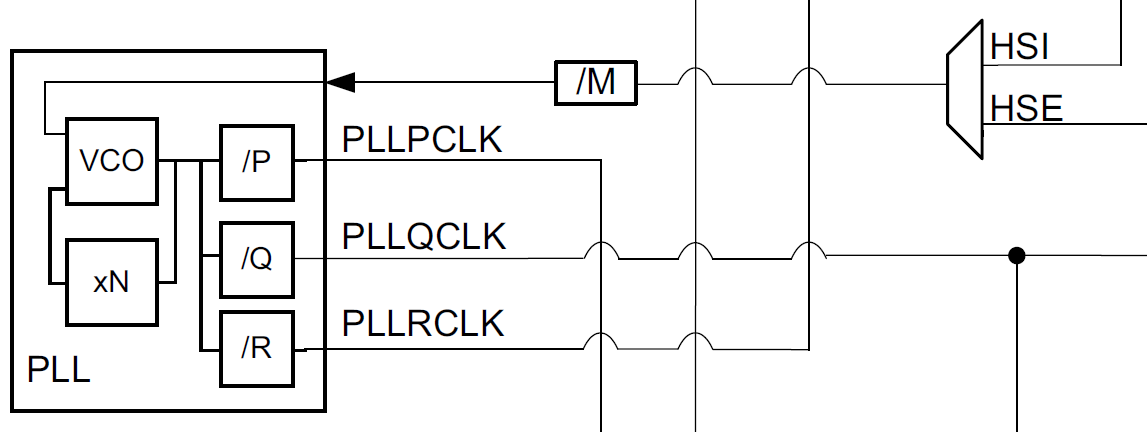
\includegraphics[width=0.6\linewidth]{Figs/Documentation/PLL_Diagram}
	\caption{Vyobrazení interního PLL bloku. Převzato z}
	\label{fig:plldiagram}
\end{figure}    

Díky této možnosti více výstupů z obvodu PLL, které mohou mít nastavené různé děličky, lze například nastavit vstupní hodiny ADC převodníku nezávisle na systémových hodinách. Toho lze vhodně využít pro optimalizaci provozních frekvencí. Například maximální frekvence vstupních hodin ADC při využití více než 1 převodníku je 52 MHz. Jelikož při odvozování frekvence ADC ze systémových hodin máme omezené možnosti předděličky, tak maximální frekvence systémových hodin by pak mohla být pouze 104 MHz. Nicméně s využitím PLL můžeme nastavit vstupní hodiny ADC převodníku na požadovaných 52 MHz a zároveň nastavit frekvenci systémových hodin na 156MHz. 

\subsection{Změna zdroje hodinového signálu systémových hodin}
Na obrázku \ref{fig:hsekonfigurace} je popsaný postup změny zdroje SYSCLK. Při změně vstupního signálu PLL nelze PLL používat, tedy je nejdříve zapotřebí přepnout systémové hodiny na interní oscilátor 16MHz. Dle doporučení v \cite{refG4} je při velkých rozdílech frekvencí mezi výstupem PLL(SYSCLK>80MHz) zapotřebí přidat mezikrok s využitím AHB předděličky hodinového signálu systémových hodin. Hodnota předděličky se nastavuje RCC\_CFGR registru. Díky tomu například ve svém programu zmenším frekvenci systémových na polovinu tedy 78 MHz a pak až nastavuji jako zdroj HSI146. Doporučená doba setrvání v tomto mezikroku je alespoň $1\mu$s. V mém řešení program čeká 1ms s využitím připravených funkcí obsahujícím čekání v jednotkách ms.


\begin{figure}[H]
	\centering
	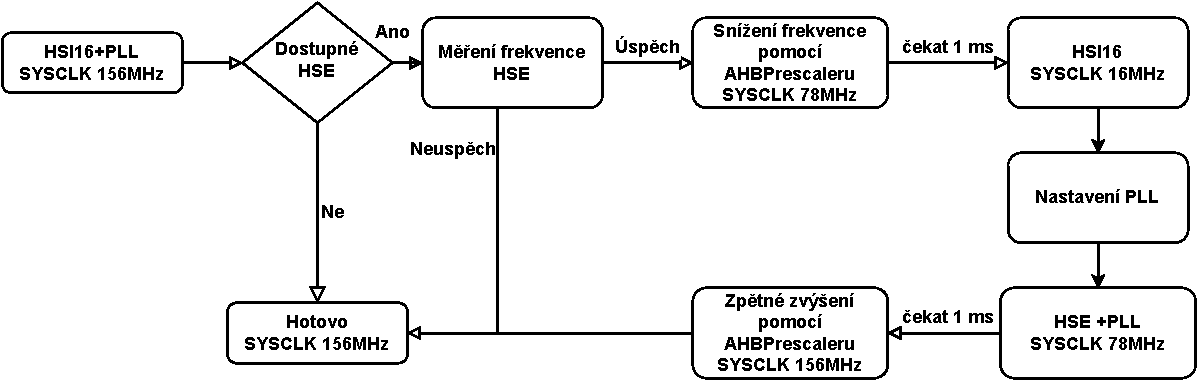
\includegraphics[width=1\linewidth]{Figs/Documentation/HSE_Konfigurace}
	\caption{Postup změny zdroje hodinového signálu}
	\label{fig:hsekonfigurace}
\end{figure}



\section{Realizace generátoru funkcí}
Součástí zadání byla implementace signálového generátoru. V práci je využit vnitřní převodník DAC pro generování jednokanálového analogového signálu s různými průběhy. Většina přístrojů do této doby implementovaných v rámci katedry měření zatím umožňovala generování pouze obdélníkové signálu s využitím PWM generátorů, které neumožňovaly některé druhy měření analogových obvodů. Zejména chyběla možnost generace sinusového signálu, který se v elektronice často využívá - například pro stanovení amplitudové a fázové frekvenční charakteristiky  RC článku. Dále generátor umožňuje generování nastavitelného stejnosměrného napětím, což dále rozšiřuje repertoár laboratorních úloh.

\subsection{Použitý DAC převodník a jeho limity}
Použitý interní DAC převodník nabízí dle \cite{dataG431} 2 výstupní kanály s maximální vzorkovací frekvenci 1 Msps a rozlišením 12 bitů. Převodník také s pouhým využitím vnitřních obvodů - tedy nezávisle na programu umožňuje generování některých signálových průběhů jako jsou trojúhelníkový signál, signál tipu "pila" či šumový signál. DAC převodník má také na svém výstupu integrovaný výstupní zesilovač, který slouží pro snížení výstupní impedance. 

\subsection{Generování signálu}
\label{ch:signalGeneration}
V předchozí části jsem zmiňoval možnost generování signálových průběhů, jako jsou  pilový nebo trojúhelníkový signál, pouze nastavením interních registrů DAC převodníku. Tato metoda spočívá v automatickém výpočtu 12 bitových hodnot pro výstup DAC převodníku prostřednictvím HW registrů. Typicky se k nastavené hodnotě(offsetu) pravidelně přičítá hodnota jiného registru s tím, že si DAC převodník sám řídí generování nových hodnot vzorků. Výhodou tohoto přístupu jsou minimální paměťové nároky, protože číslicové hodnoty jednotlivých vzorků jsou vypočtené za běhu a nejsou uloženy někde v paměti. Tohoto způsobu generování nových číslicových hodnot pro DAC převodník bylo v této práci využito pro generování pseudošumu, které popisuji v kapitole \ref{ch:noiseGeneration}\\

Nevýhodou využití interních registrů pro generaci signálových průběhů jsou především omezené možnosti ohledně změny tvaru signálu, kdy nám například chybí možnost generování sinusového signálu. Alternativou je pak uložit číslicové hodnoty v rozlišení DAC převodníku pro jednotlivé vzorky do paměti mikrokontroléru a následně prostřednictvím DMA řadiče jednotlivé vzorky posílat do DAC převodníku jako je znázorněno v obrázku \ref{fig:dacfunction}.\\

\begin{figure}[H]
	\centering
	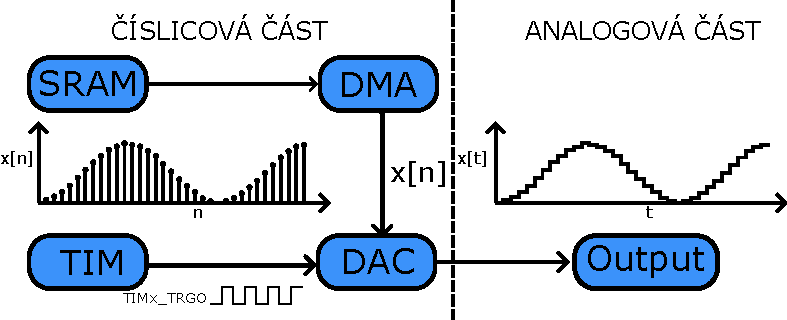
\includegraphics[width=0.9\linewidth]{Figs/Diagrams/SVG/DAC_function}
	\caption{Diagram využití DAC převodníku a dalších periferií pro generování analogového signálu}
	\label{fig:dacfunction}
\end{figure}

 Jedním z možných způsobů je uložení pevných hodnot vzorků 1 periody signálu do paměti FLASH. Hodnoty uložené ve Flash paměti, se ale za běhu složitě upravují a jako výhodnější řešení z důvodů flexibility se zdálo řešení s ukládáním hodnot vzorků do paměti SRAM. Hodnoty vzorků jedné periody můžou být tak před samotným generováním vždy přepočítány s ohledem na nastavené parametry. Pro generaci relativně hladkých průběhů signálů jsem předpokládal, že bude dostačovat maximální délka bufferu 1000 vzorků. S ohledem na maximální vzorkovací frekvenci DAC převodníku to umožňuje generování signálů s plným počtem vzorků do výstupní frekvence $f_{\text{out}}$=1 kHz.


\begin{figure}[H]
	\centering
	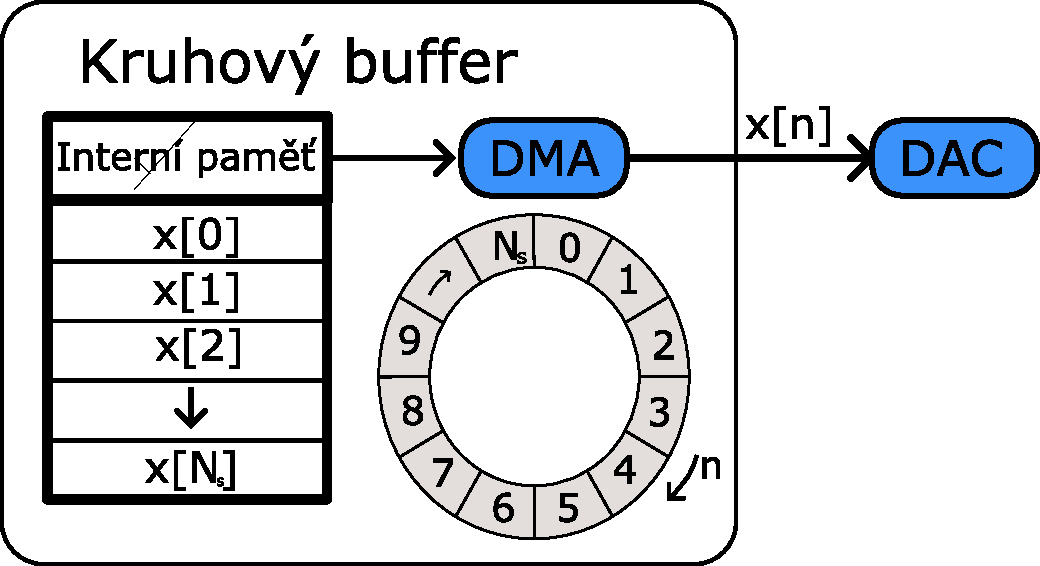
\includegraphics[width=0.55\linewidth]{Figs/Diagrams/SVG/CircularBufferDMA.pdf}
	\caption{Popis funkce kruhového bufferu jako zdroj datových vzorků pro DAC převodník}
	\label{fig:circularBuffer}
\end{figure}



\begin{figure}[H]
\begin{minipage}{0.3\linewidth}
	\centering
	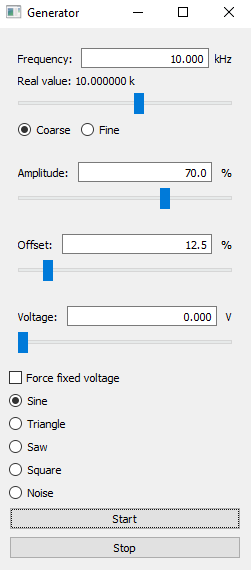
\includegraphics[width=1\linewidth]{Figs/Screenshots/ZeroElabGeneratorTab}
	\captionof{figure}{Možnosti nastavení vlastností generovaného signálu v prostředí aplikace Zero Elab Viewer}
	\label{fig:zeroelabgeneratortab}	
	
\end{minipage}
\noindent
\begin{minipage}{0.69\linewidth}	
		\begin{itemize}
			\item \textbf{Výstupní frekvence signálu} Požadovanou výstupní frekvenci signálu lze nastavovat v rozsahu 1 Hz - 250 KHz. V závislosti na nastavení výstupní frekvence signálu a omezení maximální vzorkovací frekvence DAC převodníku - se automaticky stanoví počet vzorků na jednu periodu signálu v rozsahu 4 - 1000 vzorků. 
			\item \textbf{Rozkmit} signálu se v prostředí aplikace zadává v procentech celkového 12- Bitového rozsahu DAC převodníku, který tedy jako maximální číslicovou hodnotu kterou dokáže využít bere hodnotu 0xFFF. Rozkmit určuje v jakém rozsahu se bude obor hodnot generovaného signálu pohybovat. Pokud označíme funkci určující tvar signálu $g(n)$ s tím že $n$ označuje číslo vzorku, tak můžeme psát:
			\begin{equation}
				O(g)=<0,\text{rozkmit}\times\text{0xFFF}>
			\end{equation}
			\item \textbf{Offset} nebo také posuv signálu se opět udává v procentech rozsahu převodníku. Jedná se o nejmenší hodnotu generovaného signálu respektive o hodnotu, která  posouvá vypočtené hodnoty funkcí $g$. Díky tomu můžeme popsat funkci výpočtu $n$-tého vzorku bufferu :
					\begin{equation}
				f(n)=\min{\left({(\text{offset}\times\text{0xFFF})+g(n),\text{0xFFF}}\right)}
			\end{equation}
			\item \textbf{Tvar průběhu signálu} Prostředí aplikace umožňuje zvolit různé signálové průběhy - sinusový, trojuhelníkový, signál typu pila(rampa) nebo obdélníkový.			
		\end{itemize}
		
\end{minipage}
\end{figure}

\subsubsection{Optimalizace délky bufferu}
Obvyklý postup při generaci signálu s vyžitím DMA řadiče a paměti RAM je stanovit stálý počet vzorků $N_\text{s}$ na jednu periodu generovaného signálu v závislosti na velikosti dostupné paměti. Dále na základě požadované výstupní frekvenci signálu $f_{\text{out}}$ , což je frekvence s jakou se generovaný signál má opakovat, se určí časová základna pro generování vzorků DAC převodníkem. Ta je definována dělícím poměrem DIV čítače pro generování zmíněné časové základny. Závislost tohoto dělícího poměru na frekvenci vstupních hodin toho čítače $f_{\text{PCLK}}$, výstupní frekvenci signálu a počet vzorků $N_\text{s}$ je vyjádřena vzorcem:
\begin{equation}
	\text{DIV}=\frac{f_{\text{PCLK}}}{	f_{\text{out}}\cdot }
\end{equation} 

Nicméně zde narážíme na omezené možnosti nastavení výstupní frekvence signálu v podobě dělícího poměru DIV, který může nabývat pouze celočíselných hodnot. Pro zlepšení rozmezí nastavitelných frekvencí výstupního signálu jsem se inspiroval článkem \cite{SDI_Hladik}, kde autor využívá toho, že nepracuje s konstantní délkou záznamové paměti, ale adaptivně se zkracuje pro jemné nastavení výstupní frekvence signálu. Metoda spočívá v iterativním zkracováním délky bufferu a minimalizování absolutní odchylky frekvence generovaného signálu.

V rovnicích \ref{eq:signalFrequency} uvádím vztahy pro výpočet reálné výstupní frekvence $f_{\text{out}}$, která je tedy závislá na počtu vzorků v kruhovém bufferu  ($N_\text{s}$) a vzorkovací frekvenci ($f_\text{s}$). Vzorkovací frekvence je pak zase podílem frekvence vstupních hodin čítače $f_{\text{PCLK}}$ a dělícího poměru DIV.
 
\begin{equation}
	f_{\text{out}}=\frac{f_{\text{s}}}{N_\text{s}},\quad  f_{\text{s}}=\frac{f_{\text{PCLK}}}{\text{DIV}} \quad \implies \quad f_{\text{out}}=\frac{f_{\text{PCLK}}}{\text{DIV}\cdot N_\text{s}}, \quad 
	f_{\text{s}}=\frac{f_{\text{out}}}{\text{DIV}\cdot N_\text{s}}
	\label{eq:signalFrequency}
\end{equation}

 Dělící poměr DIV je závislý na nastavení ARR (auto-reload register) a PSC(Prescaler Register) registrech čítače. Zde je podstatné uvést, že ke skutečným hodnotám registrů ARR a PSC se musí přičíst 1, abychom získali správnou hodnotu jako je vidět ve vzorci \ref{eq:DIVvalue}. Při optimalizaci délky bufferu tedy  v prvním kroku nehledáme jen dělící poměr DIV, ale faktorizaci tohoto dělícího čísla, která nám minimalizuje rozdíl mezi cílenou vzorkovací frekvencí $f_{\text{s}}$ a reálnou vzorkovací frekvencí dosažitelnou při daných vstupních hodinách čítače. Pro nalezení optimálních hodnot ARR a PSC jsem využil algoritmu popsaného v práci \cite{DujavaDIP}. 
  
  \begin{equation}
 	\text{DIV}=(\text{ARR}+1)\cdot(\text{PSC}+1)
 	\label{eq:DIVvalue}
 \end{equation}
 
 Algoritmus spočívá v iterativním zvyšování hodnoty PSC a dopočtu vhodných adeptů na ARR registr. Jeho výsledkem jsou pak 2 existující faktorizace takové, že použitím jedné faktorizace získáme frekvenci menší nebo rovnu požadované a druhou faktorizací frekvenci vyšší nebo rovnu. Porovnáním dosažitelných frekvencí pak můžeme zvolit faktorizaci, která nám zajistí menší odchylku od požadované frekvence. Kompletní popis algoritmu je dostupný v citované práci.
 
 Dále jsem při optimalizaci délky bufferu postupoval podle pseudo-kódu uvedeného v \cite{SDI_Hladik}. Nejdříve jsem určil maximální délku bufferu v závislosti na maximální vzorkovací frekvenci DAC převodníku a požadované frekvenci signálu. Následovně jsem cyklicky zmenšoval délku bufferu. Pro každou délku bufferu jsem pomocí výše již zmíněného algoritmu získal DIV a vypočítal odchylku od požadované frekvence signálu. Pokud byla odchylka menší než nejmenší zatím dosažena uloží se DIV a algoritmus pokračuje dále dokud nenastane jedna z ukončujících podmínek. Těmi je buď dosažení odchylky menší než 0,01Hz nebo zkrácení výsledné délky bufferu na 1/4 původní délky.\\
 
 Při testování funkčnosti optimalizace se potvrdila pozorování uvedené \cite{SDI_Hladik} a to, že touto metodou lze dosáhnout poměrně velké přesnosti při frekvencích do 500 Hz. S tím, jak dosáhneme frekvence 1000 Hz, tak se začne maximální velikost bufferu snižovat a  s tím se začne snižovat schopnost optimalizace frekvence signálu. Algoritmus jsem testoval za následujících podmínek:
 \begin{itemize}
 	\item Zadávané hodnoty pro požadované výstupní frekvence v rozsahu 1-10000 Hz s krokem po 1 Hz
 	\item Maximální vzorkovací frekvence DAC převodníku 1 Msps
 	\item Maximální délka bufferu - 1000
 	\item Frekvence vstupních hodin periferie čítače- PCLK 156 MHz
 	\item Změřené odchylky jsou pouze teoretické odchylky neuvažující nepřesnost frekvence krystalu.
 \end{itemize}
 
 Algoritmus jsem nechal určovat vhodné nastavení délky bufferu a dělícího poměru pro výstupní frekvence signálu s krokem po jednom Hz a ukládal maximální absolutní a relativní odchylku od požadované výstupní frekvence. Pro jednotlivé intervaly uvedené v tabulce \ref{tab:OptimalizaceFrekvence} jsem pak určil maximální odchylky a související frekvence pro které se tedy reálná výstupní frekvence nejvíce lišila od požadované. Označení $f_\text{in}$ je pro požadované výstupní frekvence a $f_\text{out}$ pak označuji reálné výstupní frekvence. 
 \begin{table}[H]

	\begin{tabular}{r|ccc|ccc}
		\multicolumn{1}{c|}{}                 & \multicolumn{3}{c|}{Maximální absolutní odchylka} & \multicolumn{3}{c}{Maximální relativní odchylka} \\ \hline
		\multicolumn{1}{c|}{Rozsah frekvencí} & $f_\text{in}${[}Hz{]}  & $f_\text{out}$ {[}Hz{]}  & Odchylka {[}Hz{]}  & $f_\text{in}${[}Hz{]} & $f_\text{out}${[}Hz{]} & Odchylka {[}\%{]} \\ \hline
		1-500 Hz                              & 477       & 477.0058         & 0,0058             & 314               & 314.0046 & 0,0015            \\
		500-1000 Hz                           & 977       & 977.0212         & 0,0212             & 977               & 977.0212 & 0,0022            \\
		1000 - 2500 Hz                        & 2361      & 2360.811         & 0,1894             & 1951              & 1951.171 & 0,0087            \\
		2500 - 5000 Hz                        & 4683      & 4683.841         & 0,8407             & 4683              & 4683.841 & 0,0179            \\
		5000 - 10000 Hz                       & 9968      & 9936.306         & 31,694             & 9968              & 9936.306 & 0,3179           
	\end{tabular}
 	\caption{Maximálních dosažené odchylky frekvencí výstupních signálů pro různá rozmezí frekvencí }
 	\label{tab:OptimalizaceFrekvence}
 \end{table}
 
\subsubsection*{Využití CORDIC}
Jak již bylo zmíněno číslicové hodnoty jedné periody průběhu se ukládají do paměti SRAM. V případě sinusového signálu je potřeba napočítat hodnoty funkce sinus v rozsahu $2\pi$ radiánů pro získání kompletní jedné periody. Pro výpočet funkce sinus v rámci kódu mikrořadiče existují různé způsoby. Běžnou variantou bývá využití standardní matematické knihovny \texttt{math.h} a její funkci \text{sinf.h}. Nicméně existují efektivnější způsoby výpočtu hodnot takovýchto funkcí například založené na HW implementaci jakou je například u STM32G431 speciálně dedikovaná periferie CORDIC.\\

CORDIC(COordinate ROtation DIgital Computer) je HW akcelerátor designovaný pro urychlení kalkulací vybraných matematických funkcí jako jsou trigonometrické a hyperbolické funkce.\cite{CORDIC}. Pro získání výsledku používá metody postupné aproximace a případě trigonometrických funkcí algoritmus konverguje pro hodnoty $-\pi$ až $\pi$ radiánů. Algoritmus využívá číselné reprezentace s pevnou řádovou čárkou.  Výpočet funkce sinu daného úhlu pak probíhá postupnými rotacemi počátečního vektoru o postupně se zmenšující úhly.S tím, že HW implementace používá pro výpočet pouze operace sčítání, posuvu a pevného scaling faktoru. Výsledek je pak připravený ve fixním počtu kroků v závislosti na požadované přesnosti výsledku. Průběh kalkulace je pak naznačen na obrázku \ref{fig:cordicoperation}. 

\begin{figure}[H]
	\centering
	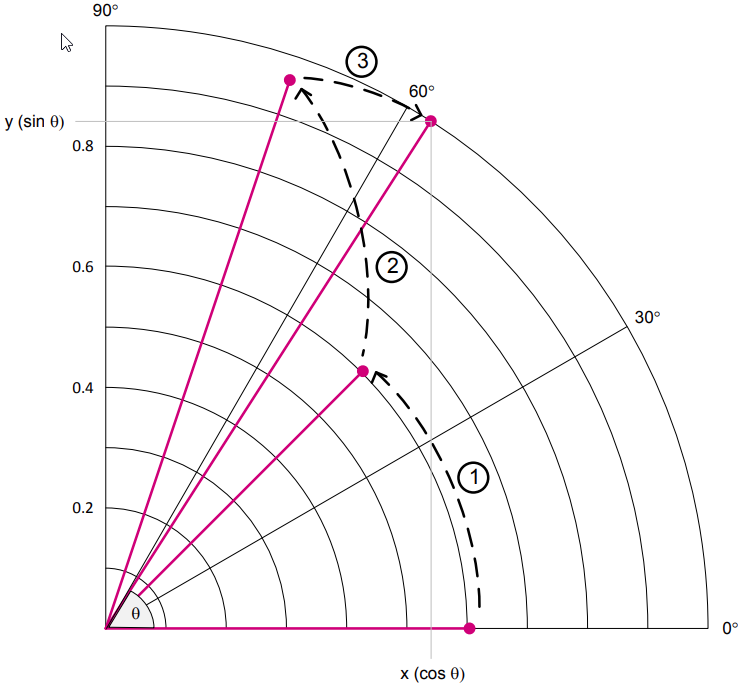
\includegraphics[width=0.5\linewidth]{Figs/Screenshots/CORDIC_Operation}
	\caption{Výpočet sinus a cosinu uhlu postupnou aproximací použitou v CORDIC převzato z \cite{AN_Cordic}}
	\label{fig:cordicoperation}
\end{figure}

Při implementaci signálového generátoru své práci jsem se snažil zjistit možný přínos využití této metody výpočtu funkce sinus. Jak již bylo zmíněno při generování signálu je zapotřebí napočítat hodnoty celého bufferu a tedy je potřeba dané matematické operace opakovat až 1000krát. Zdálo se tedy vhodné ověřit časovou náročnost výpočtu a zároveň ověřit potenciální přínos využití HW orientovaného řešení.\\

 Pro porovnání časové náročnosti výpočtu hodnot bufferu jsem zvolil podmínky, které jsou stejné s následnou implementací FW pro použití s Zero Elab aplikací. Tedy jsem porovnával za jakou dobu buffer o 1000 vzorcích přichystá MCU s využitím CORDIC a kolik času bude zapotřebí s využitím  funkce \texttt{sinf(x)} ze zmíněné standardní knihovny. Měřený úsek byl celý výpočet bufferu tedy kromě samotného výpočtu výpočty sinu postupně se zvyšující fáze, tak zároveň vynásobením spočítané hodnoty podle nastaveného rozkmitu a posun dle nastaveného offsetu. Navíc v případě použití CORDIC je nejdříve zapotřebí hodnoty převést do formátu s pevnou desetinou čárkou q1.31 a následně zpět, protože periferie s jiným formátem dat neumí pracovat. Uběhlý čas jsem pak porovnával při nastavené optimalizaci kódu se zaměřením na rychlost (-OSpeed). V tabulce \ref{tab:CordicPerformance} jsou pak srovnané dosažené výsledky.

\begin{table}[H]
	\begin{tabular}{lcc}
		\multicolumn{1}{c}{Použitá metoda} & Doba plnění bufferu  &  Čas při SYSCLK = 156MHz \\ \hline
		CORDIC                             & 37541	cyklů         &0.241 ms\\
		sinf(x) z math.h                   & 85573  cyklů  		  & 0.549 ms
	\end{tabular}
	\caption{Doba trvání přípravy bufferu o délce 1000 vzorků v závislosti na použité metodě}
	\label{tab:CordicPerformance}
\end{table}

 Z tabulky je vidět, že výpočet pomocí CORDIC byl v průměru asi o 120\% rychlejší. Nicméně obě doby výpočtu v případě využití systémových hodin s frekvencí 156 MHz jsou pod 1 ms a zřejmě tedy tyto výpočty hodnot bufferu pro DAC převodník nebudou mít žádný dopady na plynulost běhu aplikace a uživatel dobu výpočtů hodnot nijak nezaznamená. 
\subsection{Generování šumu}
\label{ch:noiseGeneration}
Pro některé experimenty v elektronice se může hodit možnost generování nastavitelného šumového signálu. Generování šumu může být využito při testování fungování obvodu za přítomnosti šumu nebo existují postupy umožňující efektivní zvýšení rozlišovací schopnosti DAC převodníků založené právě přidávání šumu do měřeného signálu. DAC převodník přítomný u MCU rodiny STM32G4 má implementován LFSR(linear feedback shift register) umožňující pomocí převodníku generování pseudo-šumu o nastavitelném offsetu a rozkmitu. Hodnota registru je vždy přepočítána po triggerování DAC převodníku podle specifického algoritmu popsaného na obrázku \ref{fig:noiselfsrcalculation}. 
\begin{figure}[H]
	\centering
	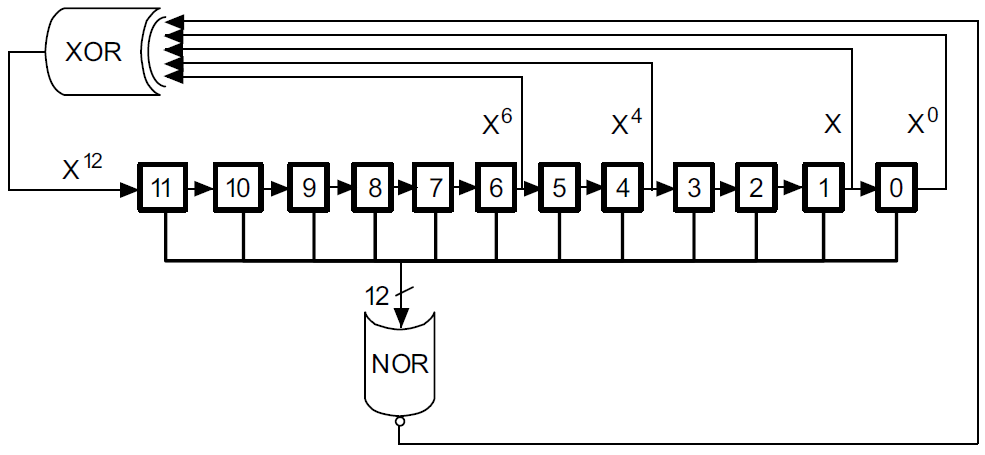
\includegraphics[width=0.7\linewidth]{Figs/Diagrams/NOISE_LFSR_Calculation}
	\caption{Naznačení průběhu výpočtu hodnot LFSR registru převzato z \cite{refG4}}
	\label{fig:noiselfsrcalculation}
\end{figure}

Samotné využití LFSR v DAC převodníku spočívá  maskováním bitů tohoto registru pro získání určitého rozmezí(rozkmitu) výstupních hodnot a následným přičtením této hodnoty získané maskováním do DHR(Data-Hold) registru. Hodnota registru DHR určuje nejmenší hodnotu posílanou na výstupu DAC převodníku - tedy offset výsledného signálu. Součet maskované hodnoty LFSR a DHR registrů se pak každý  posílá na výstup DAC převodníku (DOR registr). Celý postup je zobrazený na obrázku \ref{fig:noiseGeneration} Takto produkovaný šum má plochou spektrální distribuci a může být s určitou rezervou považován za bílý šum, s tím rozdílem, že narozdíl od pravého bílého šumu nemá Gaussovské (normální) rozdělení, ale rovnoměrné.

\begin{figure}[H]
	\centering
	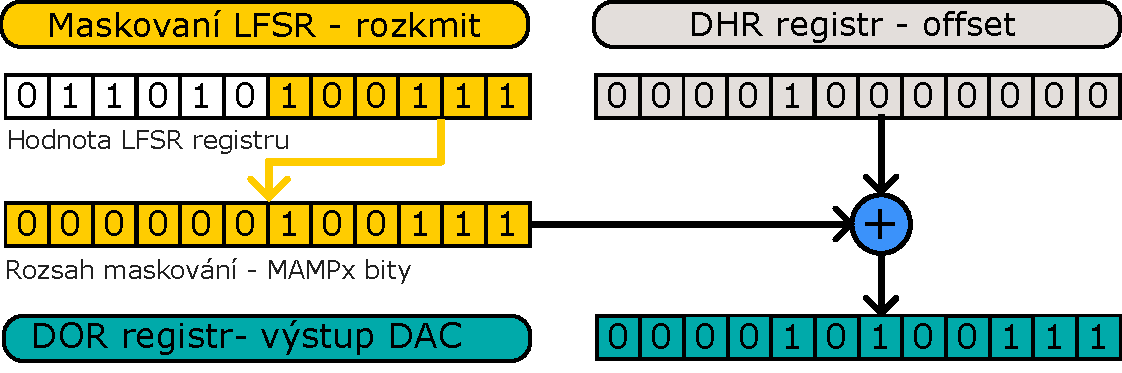
\includegraphics[width=0.7\linewidth]{Figs/Diagrams/SVG/NoiseGeneration.pdf}
	\caption{Využití LFSR registru pro generování šumu}
	\label{fig:noiseGeneration}
\end{figure}

Z obrázku \ref{fig:noiseGeneration} vyplývá jakým způsobem lze generování šumového signálu nastavovat podobně jako u ostatních tipů signálů pouze s drobnými rozdíly. Například hodnota nastavení posuvu generovaného signálu(offset) se dá nastavit v celém rozsahu DAC převodníku. Naopak menší počet různých hodnot lze nastavit pro rozkmit generovaného signálu.  Ze strany počítačové aplikace se sice zdá, že ho lze nastavovat v desetinách procenta nicméně tím, že jediný možný způsob přepočtu LFSR registru je maskováním bitů LFSR, tak lze velikost rozkmitu nastavit pouze ve 12 krocích. S tím že krok následující je polovinou kroku předchozího. Pro 50.1\% až 100\% rozkmit(a nulový offset) je na výstupu plný rozkmit šumového signálu, dalším krokem pak je rozkmit 50\% - maskujeme nejvyšší bit a a tak dále... 

\begin{figure}[H]
	\centering
	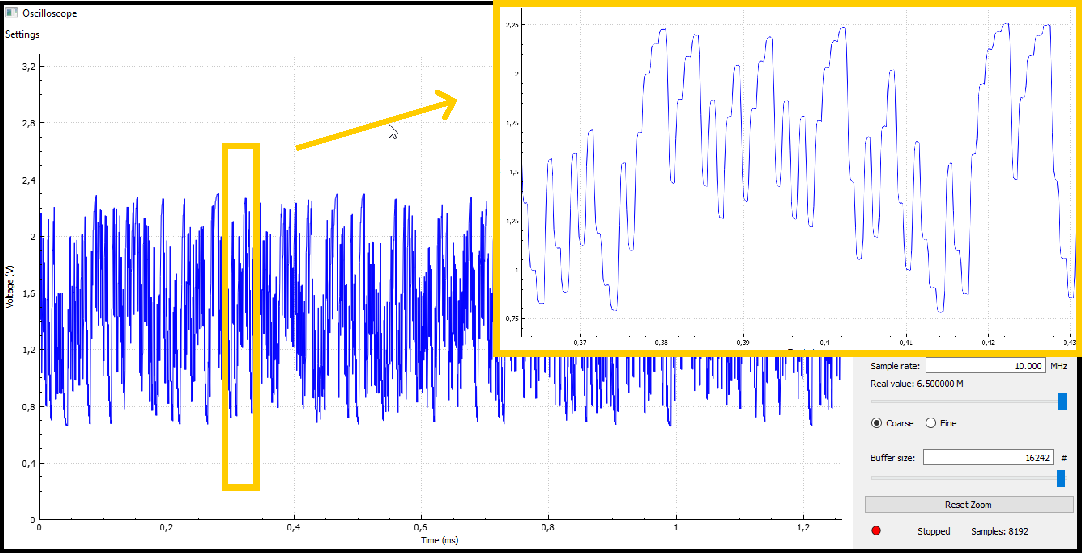
\includegraphics[width=0.8\linewidth]{Figs/Diagrams/SVG/NoiseZoom1M.pdf}
	\caption{Záznam generovaného signálu šumu se vzorkovací frekvencí 1 Msps}
	\label{fig:noiseZoom1M}
\end{figure}
Dalším nastavitelným parametrem je frekvence, která v tomto případě představuje vzorkovací frekvenci se kterou jsou nové vzorky posílány na výstup. Vzorkovací frekvence lze nastavit v rozsahu 1 Hz a 1 MHz. Nicméně vzorkovací frekvence 1MHz není pro šumový signál optimální, protože se zde začne projevovat konečná rychlost přeběhu DA převodníku zakulacováním hran jako je vidět na obrázku \ref{fig:noiseZoom1M} Pro měření  kde by se mohla projevit filtrace způsobená tímto jevem omezené rychlosti přeběhu, je lepší využít nižší vzorkovací frekvence, kde již tento problém vizualizovaný zakulacováním hran není patrný a neovlivní průběh měření. Detail generování signálu s nižší vzorkovací frekvence (250 Ksps) je vidět na obrázku \ref{fig:noiseZoom250}.
\begin{figure}[H]
	\centering
	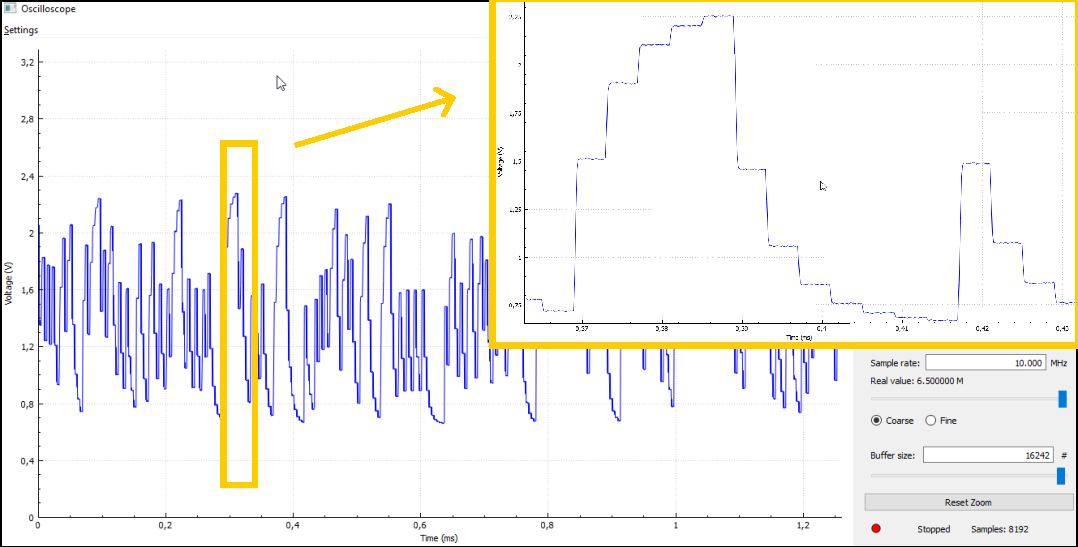
\includegraphics[width=0.8\linewidth]{Figs/Diagrams/SVG/NoiseZoom250K.pdf}
	\caption{Záznam generovaného signálu šumu se vzorkovací frekvencí 250 Ksps}
	\label{fig:noiseZoom250}
\end{figure}


\section{Realizace osciloskopu}
Modul osciloskopu je nejkomplexnějších z modulů implementovaných v této práci a též využívající nejvíce HW prostředků. K jeho implementaci jsem využil obou převodníku ADC, triggerování pomocí analog watchdog (AWDG) funkce přítomných ADC převodníků, DMA řadiče a 2 vzájemně propojených zřetězených čítačů.
\subsection{Řešení triggerování osciloskopu}
Určení okamžiku náběžné nebo sestupné hrany vstupního signálu je podstatnou funkcí osciloskopu pro zobrazování jak přechodných jevů tak periodických průběhů signálu. Existuje více přístupů, jak takovou funkci implementovat. Jednou z nejjednodušších variant je SW orientované řešení, kdy  jsou naměřená data vždy cyklicky kontrolována, zda došlo k překročení zvolené napěťové úrovně a popřípadě zastavit další sběr dat. Takové řešení bylo například použito v původní variantě FW pro STM32F042 v práci \cite{BerlingerDIP}. Nevýhodou tohoto řešení je vyšší výpočetní náročnost ve srovnání s více HW zaměřenými řešeními, jaká jsou například využití komparátorů nebo funkce AWDG, kterou disponují ADC převodníky na mikrokontrolérech STM32G4 a kterou jsem se rozhodl uplatnit v této práci já.\\

\begin{figure}[H]
	\centering
	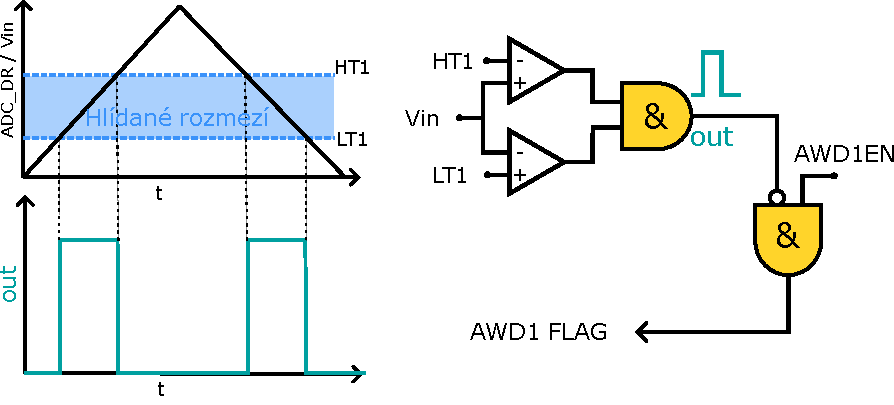
\includegraphics[width=0.9\linewidth]{Figs/Diagrams/SVG/AWD_function.pdf}
	\caption{Princip funkce Analog Watchdog(AWD) ADC převodníku}
	\label{fig:AWD_function}
\end{figure}

Blok AWDG umožňuje vyvolat přerušení v momentě, kdy se daném kanálu objeví napětí mimo nastavené rozmezí. Abychom mohli určit okamžik, kdy došlo k poklesu pod určitou úroveň(sestupná hrana) nebo naopak k překročení napěťové urovně(náběžná hrana) je potřeba využití AWDG ve dvou fázích znázorněných na obrázku \ref{fig:awdgtrigger}.

\begin{itemize}
	\item \textbf{Fáze 1}\\
	Při hledání okamžiku nástupní hrany v první fázi nejdříve nastavíme rozmezí nad střeženou napěťovou úrovní. Jakmile se napětí klesne mimo rozmezí dojde k přerušení a přesuneme se do fáze 2 
	\item \textbf{Fáze 2}\\
	V této fázi víme, že signál je pod nastavenou napěťovou úrovní. Tedy nastavíme nové střežené rozmezí napětí a víme, že jakmile dojde k přerušení, že nastal okamžik, který chceme označit jako moment nástupní hrany a uložit si číslo vzorku, kdy k tomuto došlo.
\end{itemize}
\begin{figure}[H]
	\centering
	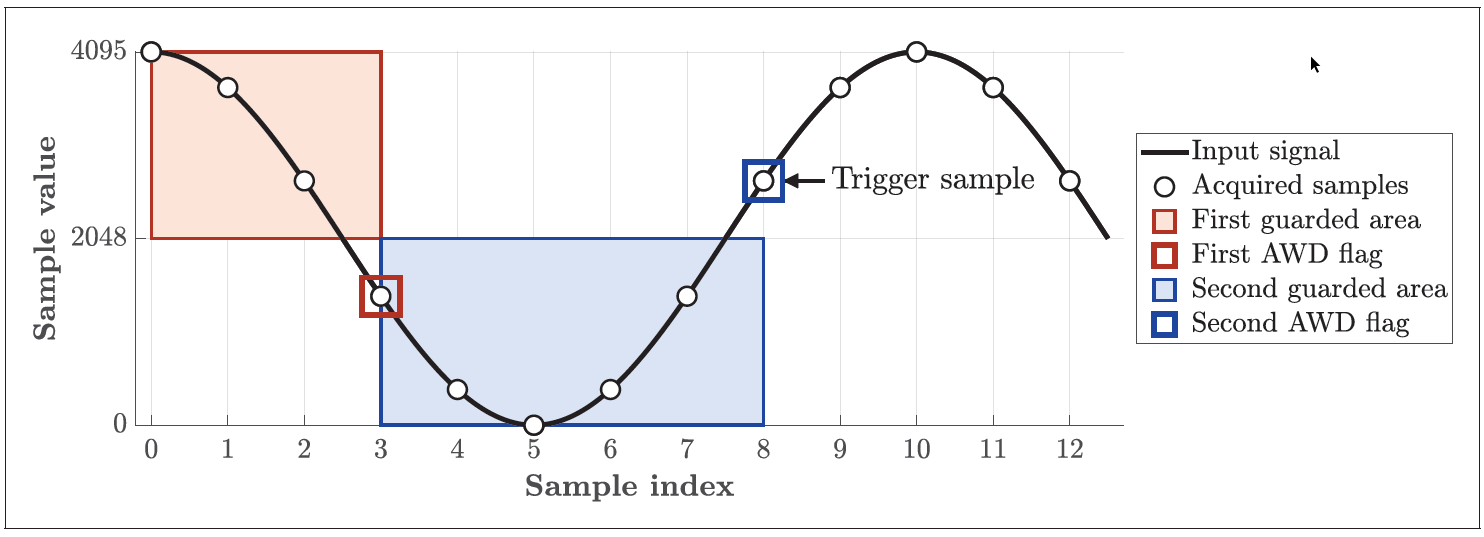
\includegraphics[width=1\linewidth]{Figs/Graphs/AWDG_Trigger}
	\caption{2-fázové triggerování na nástupnou hranu signálu s využitím AWDG- převzato z \cite{DujavaDIP}}
	\label{fig:awdgtrigger}
\end{figure}

Po vyhodnocení, že došlo k události triggeru, potřebujeme zjistit číslo vzorku, kdy moment nastal a nastavit odměření zbývajících vzorků signálů, tak aby nové vzorky zapisované do kruhového bufferu nepřepsaly data vstupního signálu před touto událostí. Zde jsem využil dvou vzájemně propojených čítačů. Funkce prvního čítače je triggerování ADC převodníku a funkce druhého čítače je počítání odměřených vzorků a poté po triggeru zastavení triggerování po daném počtu vzorků. 

\begin{itemize}
	\item \textbf{Vzorkovací čítač }\\
	Vzorkovací čítač spouští vzorkování ADC převodníku. Ve spojitosti s osciloskopy se také používá termín generátor časové základny. V závislosti na propojení interních signálů daného mikrokontroléru můžeme pro spouštění ADC buď použít nastavitelný TRGO výstup čítače nebo jeden z jeho "Capture-Compare" kanalů. V případě využití TRGO výstupu slouží UPDATE událost a kdy CNT registr dosáhne hodnoty ARR registru a čítač začíná počítat znovu od začátku. Hodnota prescaler a ARR registru tak určuje vzorkovací frekvenci. Vstupním hodinový signálem jsou interní hodiny o frekvenci systémových hodin. Navíc tento čítač operuje v slave modu "combine gated + reset", kdy tento čítač běží jen pokud na trigger vstupu(TRGI) je nastavena logická úroveň '1'. Jakmile dojde k poklesu na logickou úroveň(1), čítač se zastaví a zároveň se vyresetuje- tedy hodnota čítače CNT se vynuluje.
	
	\item \textbf{Čítač vzorků}\\
	Jak již název napovídá funkce tohoto čítače je určení pozice odebíraného vzorku v bufferu. Aktuální hodnota čítače odpovídá pozici v kruhovém bufferu následujícího snímaného vzorku. Tento čítač funguje ve funkci external clock 1, kdy čítač počítá náběžné hrany na vstupu TRGI. Na výstupu TRGO je potom stav čítače odpovídající enable bitu.
\end{itemize}

Vzájemné fungování by se pak dalo popsat následovně: pokud je zapnutý čítač vzorků, tak běží zároveň triggerovací čítač. Čítač vzorků čítá počet TRGO pulzů triggerovacího čítače a pokud čítač vzorků zastavíme, tak se zastaví triggerovací čítač a tím vzorkování ADC převodníkem. Pokud pak počítací čítač běží tzv 'one pulse' modu tak se oba čítače zastaví po odběru stanoveného počtu vzorků. 
\begin{figure}[H]
	\centering
	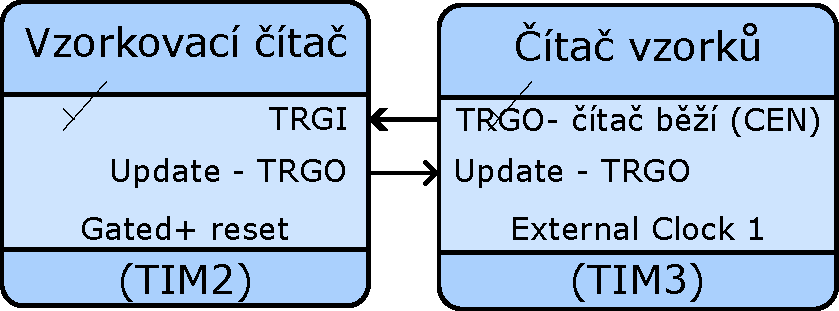
\includegraphics[width=0.5\linewidth]{Figs/Diagrams/SVG/SamplingTimerConnection.pdf}      
	\caption{Vzájemné propojení dvou čítačů}
	\label{fig:samplingtimerstrgitrgo}
\end{figure}

\subsection{Módy vzorkování}
\label{ch:ADCmux}
Pokud máme k dispozici pouze jeden ADC převodník, musíme v případě měření signálu na více kanálech vstup ADC převodníku přepínat mezi jednotlivými kanály. V případě využití dvou a více ADC převodníků máme daleko větší variabilitu, jak vzorkovat daný set analogových kanálů. Podrobněji se jednotlivým módům věnuje práce \cite{DujavaDIP}. STM32G431 má k dispozci 
2 ADC, které lze využít pro zvýšení vzorkovací frekvence, respektive zvýšení doby vzorkování pro stejnou vzorkovací frekvenci oproti použití 1 ADC. Výběr použitého módu vzorkování pak záleží na zvolených kanálech, respektive na jejich počtu a na jejich přítomnosti na jednotlivých ADC převodnících. Například kanál osciloskopu číslo 1 je na pinu PA0 a na tomto pinu také může být připojen na vstup převodníků ADC 1(kanál 1) a ADC 2(kanál1), ale například kanál osciloskopu číslo 3 je na pinu PA2, který se sice dá připojit na vstup převodníku ADC1, ale už se nedá připojit na vstup převodníku ADC2
\begin{table}[]
	\begin{tabular}{lccccc}
		Analogové kanály                & CH1         & CH2        & CH3     & CH4     & Vnitřní reference \\ \hline
		Přítomnost na Pinu               & PA0         & PA1        & PA2     & PA3     & -                 \\ \hline
		\multicolumn{1}{c}{Dostupné ADC} & ADC 1, ADC2 & ADC1, ADC2 & ADC1    & ADC1    & ADC1              \\ \hline
		Vnitřní kanál ADC                & Kanál 1     & Kanál 2    & Kanál 3 & Kanál 4 & Kanál 18         
	\end{tabular}
	\caption{Přehled jednotlivých analogových kanálů a jejich na dostupnosti na ADC převodnících}
	\label{tab:kanalyADC}
\end{table}

\begin{figure}[H]
	\centering
	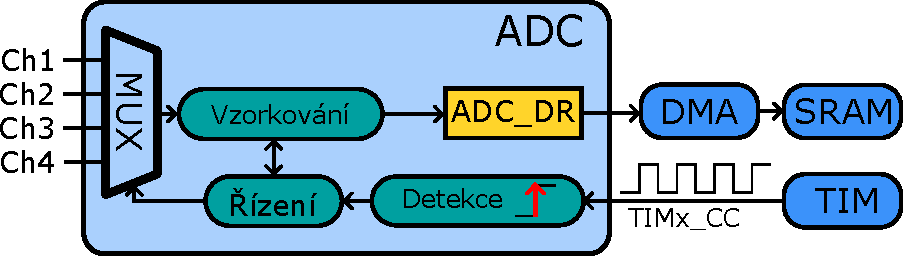
\includegraphics[width=0.7\linewidth]{Figs/Diagrams/SVG/ADC_SingleMux.pdf}
	\caption{HW konfigurace 1 ADC převodníku pro režim s multiplexováním vstupních kanálů}
	\label{HW konfigurace v případě "independent interleaved" módu}
\end{figure}

\subsubsection{Vzorkování 1 kanálu}
Pokud je zvolený analogový kanál osciloskopu  využitím vnitřních multiplexerů je možné přivést zároveň (paralelně) na vstupy obou ADC převodníků, můžeme využít tzv. "Dual -interleaved modu". Tento režim spočívá ve střídavém vzorkování jedním převodníkem a v průběhu konverze odebraného vzorku vzorkováním převodníkem druhým. U mikrokontroléru rodiny STM32G4 minimální doba odběru jednoho vzorku(vzorkování + konverze) trvá 15 period hodinového signálu ADC převodníku. V případě dual - interleaved modu lze pak vzorkovat zvolený kanál druhým ADC v momentě, kdy na prvním ADC převodníku ještě probíhá konverze. Výsledně lze pak odebrat vzorek až každých 8 cyklů. Což dovoluje téměř zdvojnásobit maximální vzorkovací frekvenci. Druhou výhodou  je možnost zvolení delší doby vzorkování při měření s nižší vzorkovací frekvencí více v kapitole \ref{Ch:SamplingTimeAndMaxInputRes}. \\

\begin{figure}[H]
	\centering
	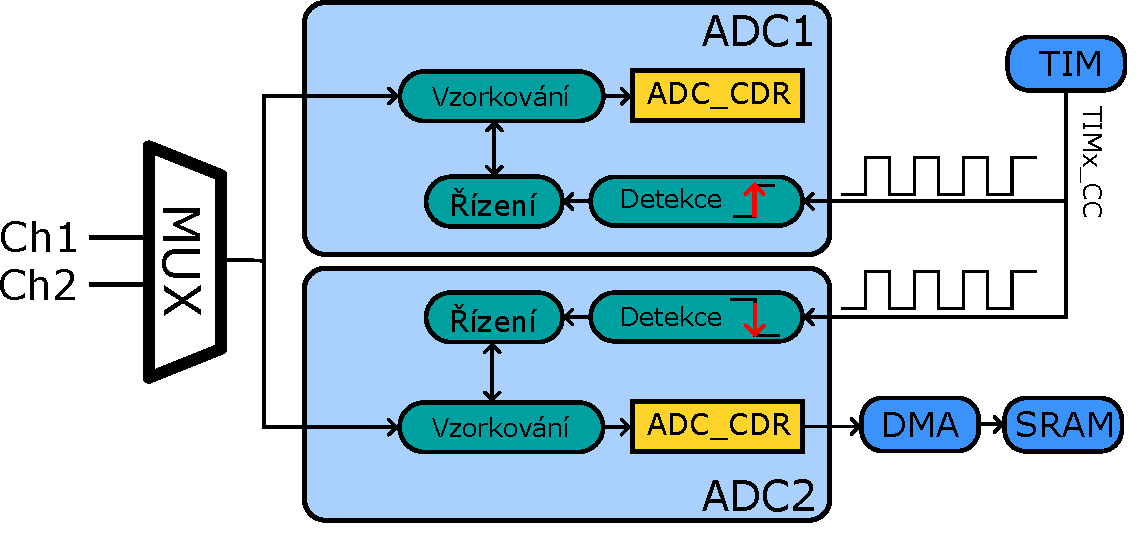
\includegraphics[width=0.8\linewidth]{Figs/Diagrams/SVG/ADC_Independent.pdf}
	\caption{HW konfigurace 2 ADC převodníků pro režim "Independent interleaved"}
	\label{fig:InterleavedHW}
\end{figure}

Nevýhodou pro STM32 ADC nativního dual interleaved režimu  je, že vzorkování podřazeného ADC2 je spuštěno pevně stanový počet cyklů po vzorkování ADC1, což může zkreslit průběh měřeného signálu, pokud časový interval mezi odběry vzorků není stejný. V mé implementaci tedy používám něco jako Independent interleaved mod. V tomto režimu využívám output compare kanálu čítače,  abych spouštěl ADC převodníky střídavě tak, aby mezi po sobě jdoucími vzorky byla pokud možno stejná vzdálenost. Na výstupu čítače tedy je nastaven obdélníkový signál se střídou 50\% , ADC1 začíná vzorkovat na hranu náběžnou a ADC2 na hranu sestupnou. Každý cyklus čítače tedy  znamená odebrání 2 vzorků. Průběh odběru vzorků je znázorněn na obrázku \ref{fig:dualinterleaved}\\

Oproti klasickému dual interleaved modu tento "independent interleaved" mód využívá nezávislého triggerování obou ADC převodníků. Nicméně stále je využito možnosti vyčítání naměřených dat ze sdílených data registrů jako v případě obvyklého 'dual-interleaved' módu. Díky využití sdílených data registrů lze snížit vytížení DMA a AHB sběrnice a vyčítat data z obou ADC převodníků najednou a to s použitím 1 DMA kanálu přenášející 32 bitů . Přenos je pak spouštěn událostí dokončení konverze na ADC2.

\begin{figure}[H]
	\centering
	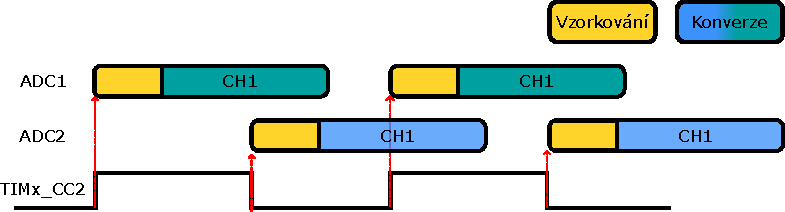
\includegraphics[width=0.9\linewidth]{Figs/Diagrams/SVG/Interleaved.pdf}
	\caption{Vzorkování v režimu "Independent Interleaved"}
	\label{fig:dualinterleaved}
\end{figure}



\subsubsection{Vzorkování 2 a více kanálů}
Pokud je to možné v případě zvolení 2 a více kanálů, je výhodné použít Dual Simultaneus režim, který nám umožní vzorkování více kanálů zároveň. V praxi nás často zajímá napětí na dvou uzlech obvodu ve stejnou chvíli. Pokud měříme pouze jedním ADC převodníkem, tak mezi odběry vzorků je měřitelné zpoždění o které bychom museli naměřená data poté korigovat.\\

Dostupnost fyzických propojení mezi piny a analogovými kanály jednotlivých ADC převodníků se mezi různými mikrokontrolery dost liší to i v závislosti na použitém pouzdře. Abych udělal firmware jednodušeji portovatelný na další zařízení, tak jsem mém FW implementoval automatické přiřazování kanálů jednotlivým převodníků, podle jejich dostupnosti. Přiřazování probíhá tak, že nejdříve se přiřadí kanály, které jsou dostupné pouze na jednom z převodníků a pak se posloupnosti kanálů doplní kanály dostupnými na obou převodnících tak, aby pokud možno oba ADC převodníky snímaly stejný počet kanálů. Vznikají tak různé konfigurace na základě zvolených kanálů.\\

Při analogových kanálech, tak jak jsou popsány v tabulce \ref{tab:kanalyADC},je při zvolení jakýkoliv 2 kanálů CH1-CH4 zajištěno snímání ve stejný čas, kromě kombinace CH3+Ch4, které jsou oba dostupné pouze na ADC1 a tedy musí být vzorkovány multiplexováním vstupu ADC převodníku. To má za následek v případě této kombinace sníženou maximální vzorkovací frekvenci v porovnání s jinými 2 kanálovými konfiguracemi. V případě zvolení 3 nebo 4 kanálů se pak ukázalo jako nejvhodnější řešení pevné nastavení skenování všech 4 kanálů, kdy jsou najednou snímány kanály CH1+CH3 a CH2+CH4. Po navzorkování bufferu je pak případně nezvolený kanál vyfiltrován z bufferu před posláním naměřených dat do počítače.\\

\begin{figure}[H]
	\centering
	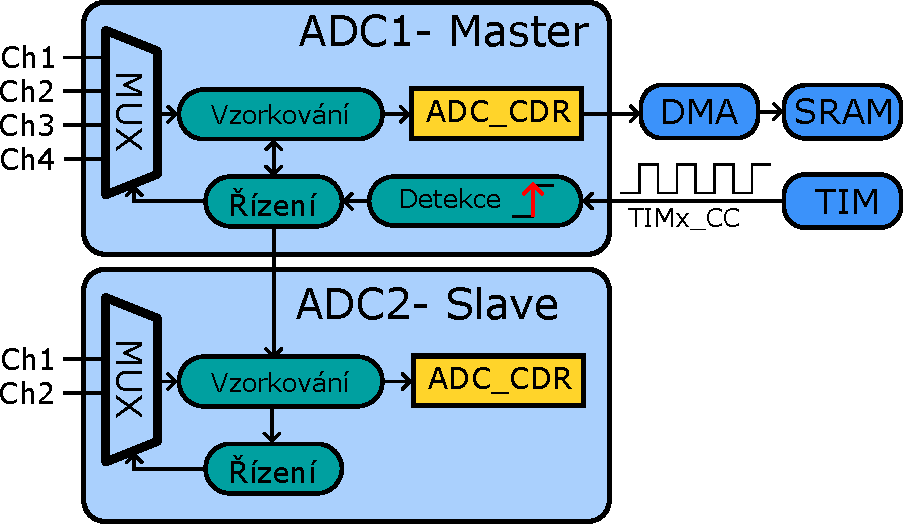
\includegraphics[width=0.6\linewidth]{Figs/Diagrams/SVG/ADC_Dual.pdf}
	\caption{HW konfigurace 2 ADC převodníků pro režim "Dual simultaneous"}
	\label{fig:dualSIMUL}
\end{figure}

Samotné používání 2 ADC převodníků využívá pro STM32 ADC nativního DUAL simultaneous režimu řízení vzorkování. V tomto režimu spouštíme vzorkování pouze řídícího(MASTER) ADC převodníku, který sám řídí podřazený ADC převodník. HW konfigurace včetně zbylých periferií je ukázána na obrázku \ref{fig:dualSIMUL}. V tomto režimu se také podobně jako je tomu u interleaved režimnu používá společného data registru(CDR), díky čemuž můžeme naměřená data z obou převodníku přenést pomocí DMA řadiče najednou.

Pokud sbíráme data z 4 analogových kanálů najednou je zapotřebí použít vnitřních multiplexerů ADC převodníku jako je tomu v případě více kanálů na jednom ADC převodníku. Průběh vzorkování pro 4 kanály je ukázán obrázku \ref{fig:dualsimul2adc}. Je patrné, že se kanály CH2 a CH4 budou nutně zpožďovat za kanály CH1 a CH3. Toto zpoždění je závislé na době vzorkování, kterou v rámci své práce upravuji na základě zvolené vzorkovací frekvence, tak aby doba odběru vzorku byla pokud možná nejdelší. 

\begin{figure}[H]
	\centering
	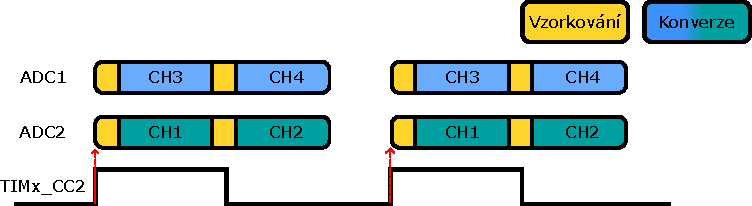
\includegraphics[width=0.9\linewidth]{Figs/Diagrams/SVG/DualSimul.pdf}
	\caption{Vzorkování 4 kanálů v režimu "Dual simultaneous"}
	\label{fig:dualsimul2adc}
\end{figure}

V běžném režimu vzorkování si zpoždění odběru vzorku pravděpodobně nevšimneme, protože zpoždění bude typicky menší než doba která uběhne mezi 2 po sobě jdoucími odběry. Nicméně zpoždění je velmi patrné při vzorkování v ekvivalentním čase. Na obrázku \ref{fig:dualsimul4chn} je vidět příklad vzorkování s ekvivalentní vzorkovací frekvencí 52 MHz. Zpoždění mezi kanály je v tomto případě rovno $N_{\text{Delay}}=653$ cyklů ADC převodníku, což při frekvenci hodin ADC převodníku $f_{\text{ADC}}=52$ MHz odpovídá zpoždění $T_{\text{Delay}}=12.55\mu$s

\begin{equation}
	T_{\text{Delay}}=\frac{N_{\text{Delay}}}{f_{\text{ADC}}}=\frac{653}{52 \text{MHz}}=12.5\mu\text{s}
\end{equation}

Na vstup byl při tom přiveden obdélníkový signál s frekvencí 10000 KHz, jehož perioda T=10$\mu$s. Tedy zpoždění signálu je o více než jednu periodu snímaného signálu. Pokud bychom tedy chtěli například měřit zpoždění signálu na nějakých logických obvodech, tak je potřeba vzít existenci tohoto zpoždění v potaz a nebo použít kanály, které jsou vzorkované zároveň.


\begin{figure}[H]
	\centering
	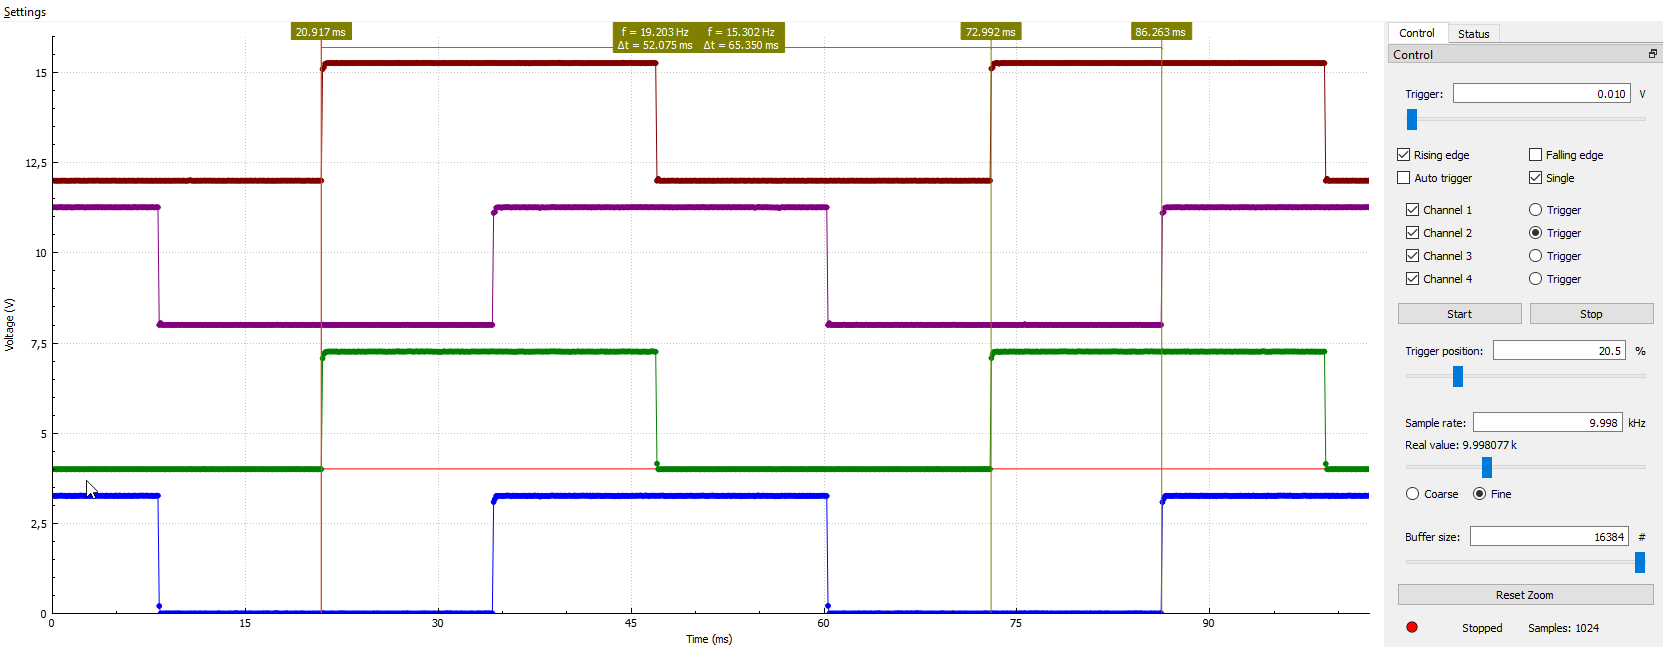
\includegraphics[width=1\linewidth]{Figs/Screenshots/DualSimul4Chn}
	\caption{Zpoždění kanálu 2 a 4 za kanálem 1 a 3 při použití Dual simultaneus modu a stroboskopickém vzorkování s ekvivalentní vzokovací frekvencí 52MHz}
	\label{fig:dualsimul4chn}
\end{figure}

\newpage
\subsection{Nastavení délky vzorkování a vliv na maximální vstupní odpor}\label{Ch:SamplingTimeAndMaxInputRes}
Impedance analogového zdroje signálu, respektive sériový odpor($R_\text{AIN}$) mezi zdrojem a pinem, ovlivňuje proud nabíjející vzorkovací kondenzátor. Časová konstanta nabíjení $t_c$ potom určuje minimální dobu vzorkování $T_s>tc$, tak aby se vzorkovací kondenzátor měl čas nabít  na vstupní napětí(s tolerancí 1/2 LSB) $V_\text{AIN}$ jako je znázorněno na obrázku \ref{fig:samplingtimeandmaxinputresistance}. 

\begin{equation}
	t_c=(R_\text{ADC}+R_\text{AIN})\times C_\text{ADC}, \quad T_s=\frac{N_{\text{s}}}{f_\text{ADC}} 
	\label{eq:RAIN}
\end{equation}


\begin{figure}[H]
	\centering
	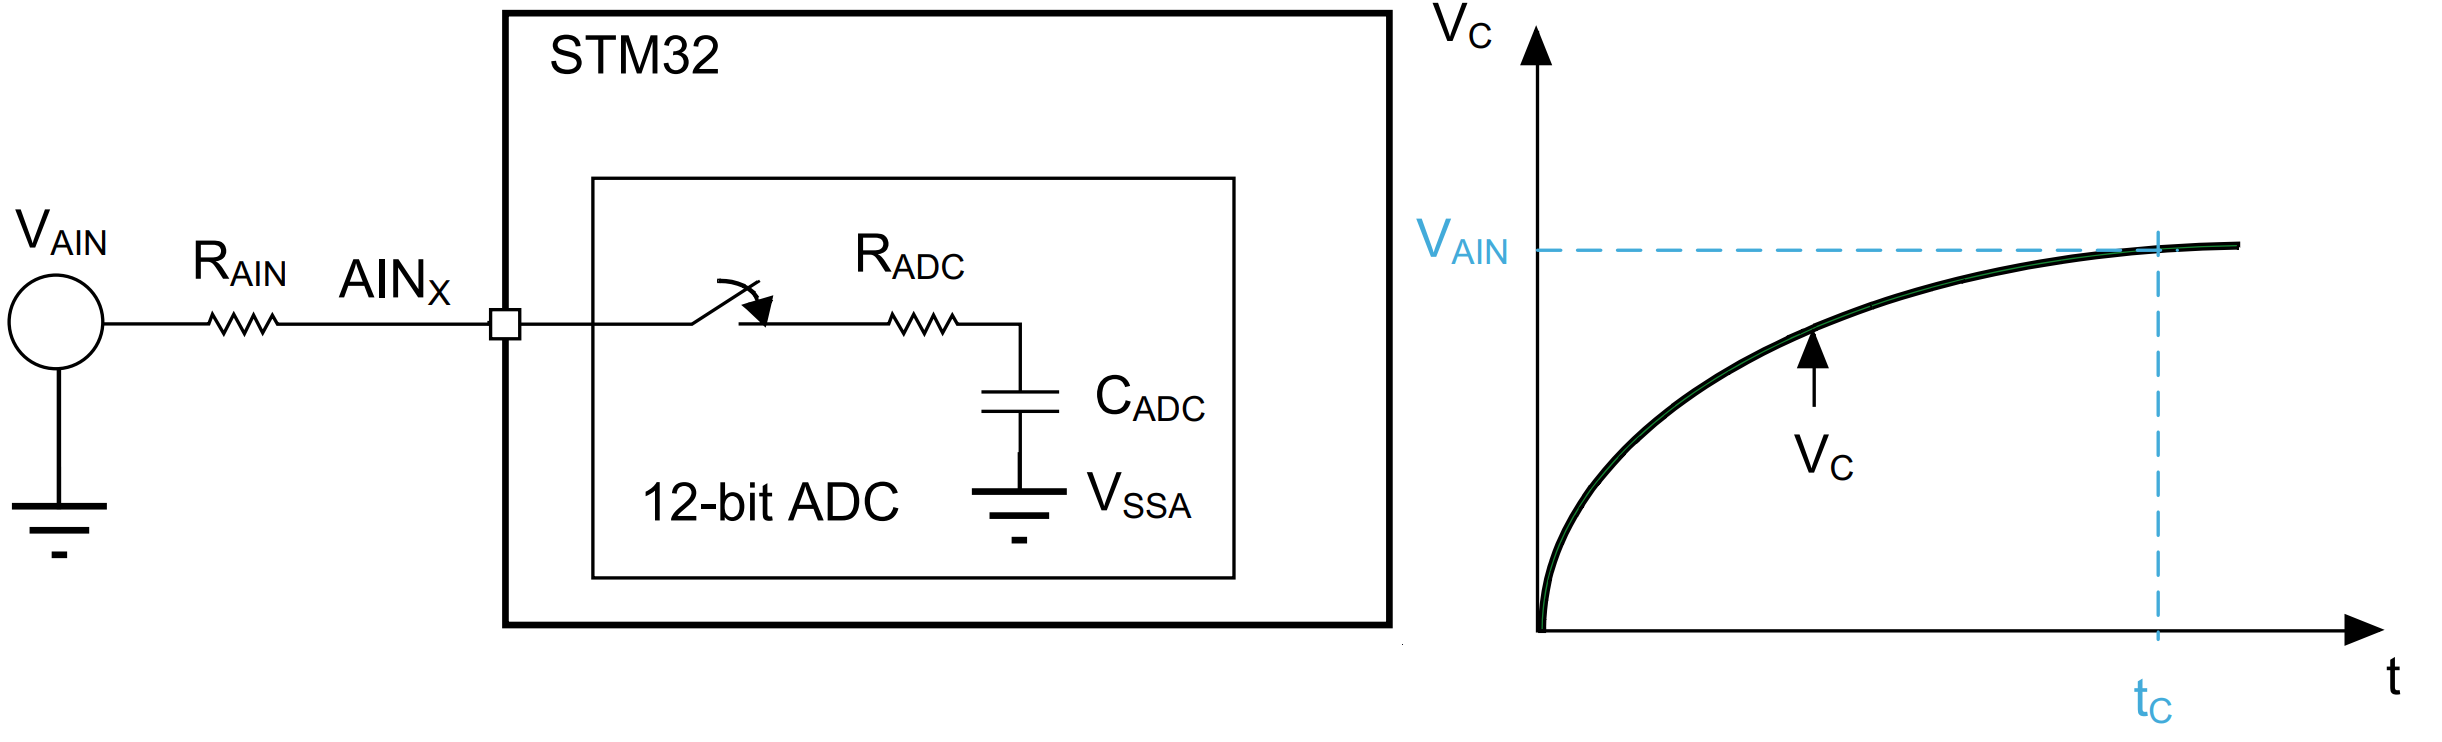
\includegraphics[width=0.9\linewidth]{Figs/Diagrams/SamplingTimeAndMaxInputResistance}
	\caption{ převzato z \cite{ADC_Acuraccy}}
	\label{fig:samplingtimeandmaxinputresistance}
\end{figure}

Doba vzorkování $T_s$ je určena počtem cyklů doby vzorkování $N_{\text{s}}$ hodinového signálu ADC (ADC\_CLK) převodníku, jehož frekvenci označuji $f_\text{ADC}$. Typicky je pro daný ADC převodník omezený výběr hodnot $N_{\text{s}}$, které jsou k dispozici. V případě STM32G431 se jedná o výběr 8 různých hodnot viz tabulka \ref{tab:maxRAIN}. Kromě zvolení hodnoty $N_{\text{s}}$, lze ovlivnit dobu vzorkování  $T_s$ také změnou frekvence $f_\text{ADC}$.\\

Při řešení osciloskopu jsem zvolil frekvenci ADC\_CLK jako maximální doporučenou frekvenci při používání 2 ADC převodníků zároveň $f_\text{ADC}=52$MHz dle technické specifikace uvedené v \cite{dataG431}. $N_s$ je ve FW přizpůsobovaná aktuální vzorkovací frekvenci $f_{\text{SAMP}}$ takovým způsobem, aby se všechny aktuálně zvolené kanály stihly navzorkovat a zkonvertovat před tím, než přijde z čítače časové základny pokyn k dalšímu odběru vzorků.\\

Výběr vhodného počtu cyklů doby vzorkování $N_s$ pro danou vzorkovací frekvenci $f_s$ probíhá následovným způsobem. Máme nějaký počet dostupných ADC cyklů pro odběr a konverzi vzorků $N_{\text{available}}$ a  celkový potřebný počet cyklů pro odběr vzorků $N_{\text{total}}$ pro které platí:
	
\begin{equation}
N_{\text{total}}=(N_s+N_c)\times N_{\text{ch}}, \quad N_{\text{available}}=\frac{f_\text{ADC}}{f_{\text{SAMP}}}
\end{equation}
kde $N_c=12.5$ označuje potřebný počet cyklů ADC převodníku pro konverzi 12-bitové naměřené hodnoty a $N_{\text{ch}}$ označuje kolik kanálů vzorkuje 1 ADC převodník v případě multiplexování kanálů. Následně volíme hodnotu $N_s$ ze seznamu dostupných hodnot tak, aby byla bylo dosaženo maximální možné doby vzorkování $T_s$ aniž by došlo k překročení dostupného počtu cyklů $N_{\text{total}}$. Doba vzorkování ovlivňuje měření a pro uživatele může být výhodné tuto informaci znát. Z tohoto důvodu po zvolení počtu cyklů MCU informuje uživatele skrz PC aplikaci formou informace o maximální impedanci zdroje signálu aby byla dodržena podmínka uvedená v \ref{eq:RAIN} a doba vzorkování $T_s$ delší než velikost časové konstanty nabíjení vnitřního vzorkovacího kondenzátoru $t_c$.

Zmíněný vzorec je vhodné použít pokud známe přesné vnitřní parametry ADC převodníku. Ty v mém případě nebyli známy a z dat v datasheetu STM32G431 vyplívá, že například hodnota vnitřního odporu ADC převodníku $R_{\text{ADC}}$ se mění v závislosti na konfiguraci. Pro určení maximální vstupního odporu pro danou dobu vzorkování $T_s$ jsem tedy místo vzorce použil hodnoty uvedené v datasheetu\cite{dataG431}. V mé implementaci byli využity tzv."Fast channels", což jsou vnitřní kanály 1 až 5 ADC převodníku, které umožňují vzorkování vstupů s daným vnitřním odporem v kratším čase. V tabulce \ref{tab:maxRAIN} pak uvádím přehled hodnot maximálního vstupního odporu v souvislosti se zvolenou dobou vzorkování. Na základě této tabulky a informace z aplikace o maximálním vstupním odporu pak uživatel může určit použitou dobu vzorkování.\\

\begin{table}[H]
	\begin{tabular}{lrrrrrrrr}
		Max $R_{\text{AIN}}$ [$\Omega$]       & \multicolumn{1}{c}{100} & \multicolumn{1}{c}{330} & \multicolumn{1}{c}{680} & \multicolumn{1}{c}{1500} & \multicolumn{1}{c}{2200} & \multicolumn{1}{c}{4700} & \multicolumn{1}{c}{12000} & \multicolumn{1}{c}{39000} \\ \hline
		$N_{\text{s}}$ & 2.5                     & 6.5                     & 12.5                    & 24.5                     & 47.5                     & 92.5                     & 247.5                     & 640.5                     \\
		$T_s$ {[}ns{]}    & 48                      & 125                     & 240                     & 471                      & 913                      & 1779                     & 47660                     & 12317                    
	\end{tabular}
	\caption{Přehled hodnot maximálního vstupního odporu společně s odpovídající dobami vzorkování}
	\label{tab:maxRAIN}
\end{table}

 Na obrázku \ref{fig:wrongmaxrain} je pak vyobrazen příklad, kdy pomocí impulzního generátoru generuji PWM signál s frekvencí $f_{\text{pwm}}=$5 kHz a přivádím na vstupy ADC převodníků. Jeden z kanálů je připojen na přímo a druhý kanál přes odpor 47 k$\Omega$. Pro vzorkovací frekvenci $f_{\text{SAMP}}=2$MHz dostaneme informaci o maximálním vstupním odporu $R_{\text{AIN}}=680\Omega$. Odpovídající dle tabulky \ref{tab:maxRAIN} době vzorkování $T_s=240$ ns. Na vstupním kanálu číslo 1, který je spojen se impulzním generátorem přes zmíněný odpor R=47 k$\Omega$ je vidět pokles napětí $\Delta V=691$ mV způsobený tím, že se vzorkovací kondenzátor se nestíhá dobíjet nedodržením podmínky \ref{eq:RAIN}.


\begin{figure}[H]
	\centering
	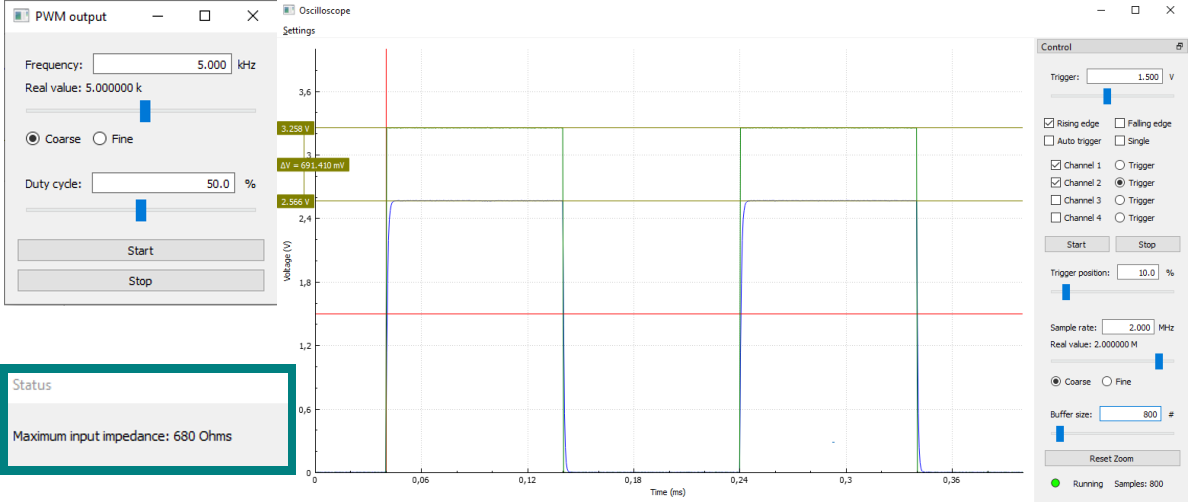
\includegraphics[width=0.9\linewidth]{Figs/Screenshots/RAINpwmgraph.pdf}
	\caption{Efekt nedodržení maximálního vstupního odporu}
	\label{fig:wrongmaxrain}
\end{figure}

\newpage
\section{Logický analyzátor}
Logický analyzátor nahrazuje funkci osciloskopu pro sledování logických signálů, jakými jsou například signály sériových sběrnic typu UART nebo I2C. V případě osciloskopu máme velmi omezený počet kanálů, které můžeme vzorkovat zároveň daný počtem dostupných ADC převodníků. Tento problém sice můžeme řešit multiplexováním vstupních kanálů, jak bylo popsáno kapitole \ref{ch:ADCmux} nicméně to má zase velký vliv na maximální vzorkovací frekvenci. Zároveň nutnost vzorkování a následné konverze dále zpomaluje celé vyčítání stavu logického kanálu.\\
\begin{figure}[H]
	\centering
	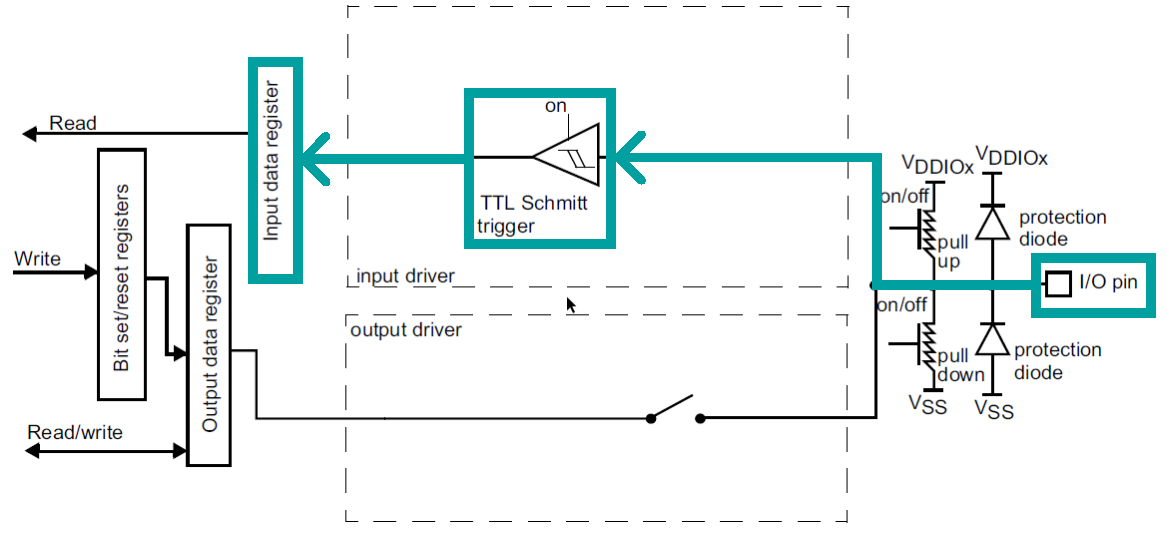
\includegraphics[width=0.8\linewidth]{Figs/Diagrams/SVG/InputPin.pdf}
	\caption{Vnitří struktura pinu v "Input" konfiguraci. Převzato z \cite{refG4}}
	\label{fig:GpioINPUT}
\end{figure}
Díky tomu, že u logických kanálů rozlišujeme jen 2 napěťové úrovně, tak ADC převodník pro určení stavu kanálu nepotřebujeme a stačí využít vnitřní struktury vstupních pinů (Obr. \ref{fig:GpioINPUT}). Součástí této struktury je registr vstupních dat(GPIO\_IDR), který zachycuje stav I/O pinu každou periodu hodin AHB sběrnice. Tento registr pak obsahuje stav všech pinů náležící k jedné GPIO bráně a za předpokladu, že jsou sledované vstupy v rámci jedné GPIO brány, tak můžeme vyčíst stav všech vstupů zároveň jedním přístupem do registrů.

\begin{figure}[H]
	\centering
	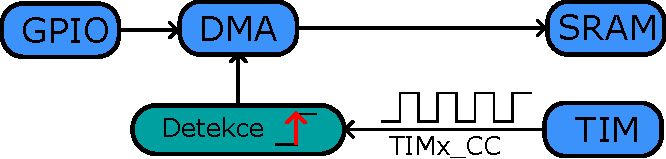
\includegraphics[width=0.6\linewidth]{Figs/Diagrams/SVG/LogicAnalyzer.pdf}
	\caption{HW konfigurace pro logický analyzátor}
	\label{fig:LogicAnalyzerHW}
\end{figure}
 Pro synchronní vyčítání registru GPIO\_IDR můžeme efektivně využít DMA řadiče ve spojení s čítačem podobně jako v případě osciloskopu. Čítač pak určuje časovou základnu pro odběr vzorků řídí přenosy hodnot registru do bufferu v SRAM paměti. Tato propojení periferií je znázorněno na obrázku \ref{fig:LogicAnalyzerHW}. 

Maximální vzorkovací frekvence, kterou jsme schopni snímat vstupy logického analyzátoru je limitována rychlostí DMA přenosu. DMA přenos typicky trvá 6 cyklů hodin AHB sběrnice \cite{AN_DMA}. S tím, že přenos může trvat déle v případě souběžných přístupů do SRAM paměti nebo v případě vytíženosti AHB sběrnice dalšími procesy. Z tohoto důvodu jsem pro přenos počítal $N_{\text{DMA\_cyklů}}$= 8 cyklů, abych snížil vytížení sběrnice a nedocházelo ke kolizím. Maximální vzorkovací frekvence $f_{s}$ logického analyzátoru je tedy určena při dané frekvencí hodin AHB sběrnice $f_{\text{HCLK}}$ jako:

\begin{equation}
	f_{s}=\frac{f_{\text{HCLK}}}{N_{\text{DMA\_cyklů}}}=\frac{156 \text{ MHz}}{8}=19.5\text{ MHz}
\end{equation}

 Maximální vzorkovací frekvence až 19,5 MSps, je dostatečná pro řadu využití jako je například analýza sériové komunikace pomocí I2C, UART nebo SPI, se kterými se studenti v hodinách běžně potkávají.

\begin{figure}[H]
	\centering
	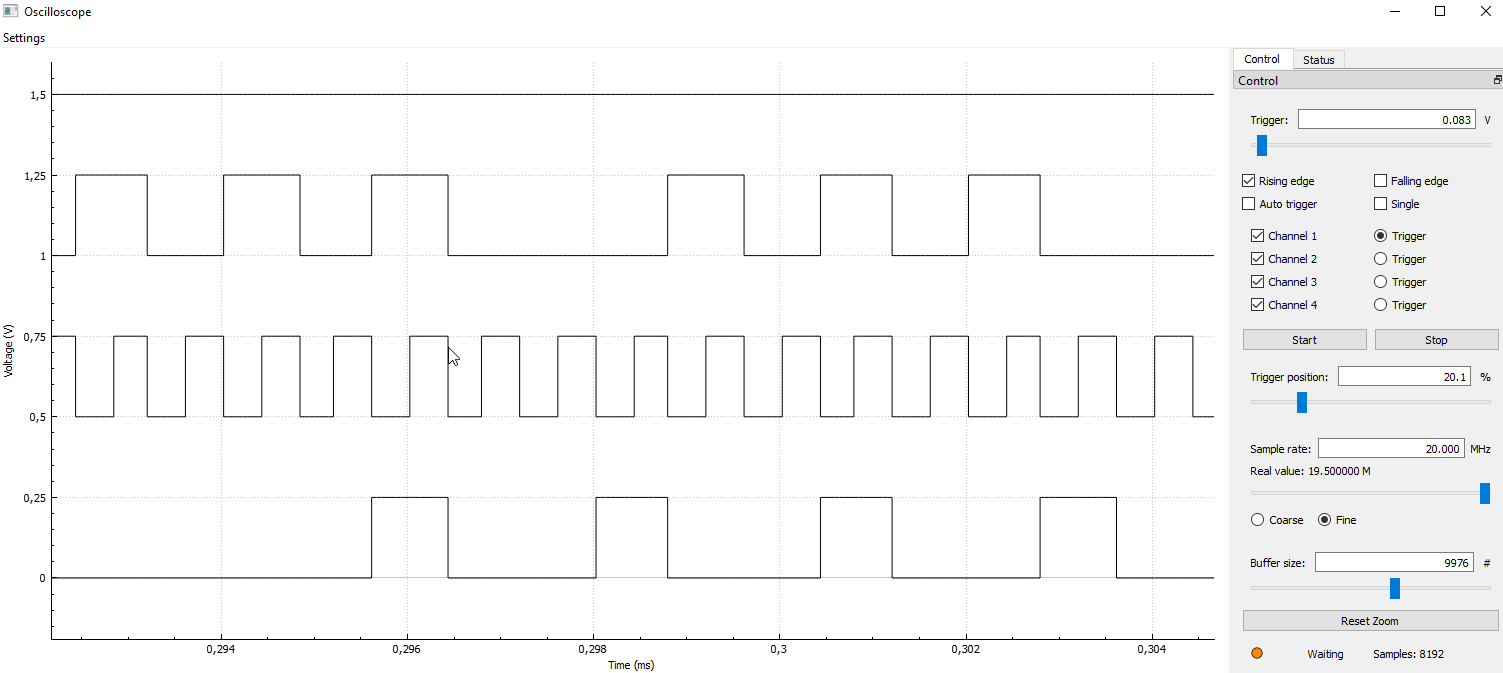
\includegraphics[width=1\linewidth]{Figs/Screenshots/SPICommunicationLogicAnalyzer.png}
	\caption{Záznam SPI komunikace s baudrate = 125 KBits/s}
	\label{fig:LogicAnalyzerSPIrecord}
\end{figure}

\subsection{Triggerování logického analyzátoru pomocí externího přerušení - EXTI}
Podobně jako u osciloskopu je i u logického analyzátoru potřeba triggerování záznamu některým ze zvolených signálů. Narozdíl od osciloskopu se v případně logických signálů nemusí vyhodnocovat úrovně napětí, ale rozhodující úlohu hrají náběžné nebo spádové hrany. Pro tento účel lze velmi účelně využít dostupnou řídící jednotku pro přerušení a události - EXTI (extended interrupts and events controller). Tato řídící jednotka slouží jako prostředník mezi periferiemi a řídicí jednotkou přerušení (NVIC). Díky tomu stejný signál, který využíváme jako vstupní může tak zároveň sloužit jako signál přerušení. V momentě, kdy na zvoleném vstupním signálu dojde ke změně napěťové úrovně - tedy k náběžné nebo sestupné hraně(podle volby) vstupního signálu, tak dojde k vyvolání přerušení běhu programu.
\begin{figure}[H]
	\centering
	\includegraphics[width=1\linewidth]{Figs/Diagrams/SVG/EXTI}
	\caption{EXTI blokový diagram - konfigurace vyvolání přerušení daným pinem - převzato z \cite{G4EXTI}}
	\label{fig:exti}
\end{figure}

Po vyhodnocení události přerušení pak dojde přenastavení čítače, který počítá odebrané vzorky, tak aby odebral zbývající počet vzorků $N_{\text{posttrigger}}$ a následně zastavil měření. $N_{\text{posttrigger}}$ se odvíjí od celkové délky bufferu $N_s$ a zadané hodnoty pre-triggeru v procentech.
\begin{equation}
	N_s=N_{\text{pretrigger}}+N_{\text{posttrigger}}, \quad N_{\text{pretrigger}}=\text{Pretrigger[\%]} \times N_s, \quad N_{\text{posttrigger}}=N_s \times(1-\text{Pretrigger[\%]} )
\end{equation} 

\begin{figure}[H]
	\centering
	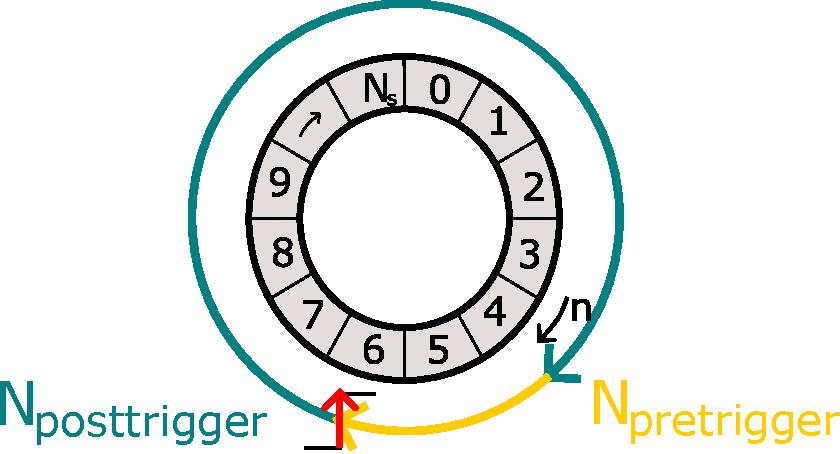
\includegraphics[width=0.6\linewidth]{Figs/Diagrams/SVG/CircularPostTrigger.pdf}
	\caption{Rozdělení kruhového bufferu na data před a po přerušení}
	\label{fig:exti}
\end{figure}

 V rámci mého řešení takto lze triggerovat záznam logického analyzátoru pomocí jednoho ze 4 různých vstupních kanálů s tím, že lze zvolit chceme-li triggerovat na náběžnou hranu, sestupnou hranu nebo obě, kdy jakákoli hrana, která dorazí na vstup zvoleného signálu vyvolá přerušení. Díky implementaci pretriggeru lze pak sledovat co se odehrávalo na vstupech před vyvoláním přerušením.
 
 \newpage
 \section{Realizace funkce čítač - měření frekvence a střídy}
 Přístroj typu čítač s funkcí měření frekvence vstupního signálu se hodí v mnoha případech. Pokud například chceme využít osciloskopu v režimu vzorkování v ekvivalentním čase, tak potřebuje znát přesnou frekvenci vstupního signálu, abychom mohli správně zvolit vzorkovací frekvenci osciloskopu. Využitím vnitřních periferií čítačů pro měření frekvence vstupních signálů navíc můžeme měřit větší rozsah frekvencí než například interpretací naměřených dat z osciloskopu, kde jsme limitováni vzorkovací frekvencí ADC převodníku. Kromě měření frekvence lze vnitřních čítačů využít i například pro měření střídy vstupního signálu. V rámci této práce jsem adaptoval 2 různé postupy pro měření frekvence s tím že mezi způsoby měření si v aplikaci můžeme vybrat.\\
 
 Reciproční metoda měření frekvence,  která spočívá v měření délky periody se hodí více pro pomalejší signály a v rámci mé implementace navíc umožňuje měření střídy signálu. Druhou metodou, kterou jsem se v této práci zabýval je metoda čítáním pulzů. která se naopak hodí více pro
 
 \subsection{Reciproční metoda měření frekvence určením délky periody - PWM input režim}
 Upravenou verzi metody měření délky periody vstupního signálu popsané v kapitole \ref{ch:HSEFrequencyMeas}, můžeme využít pro stanovení vlastností PWM signálu. Kromě určení délky periody  tak lze čítač využít i k určení střídy PWM signálu. Metoda je popsaná v \cite{refG4} a označována jako PWM input režim. Režim spočívá v konfiguraci čítače v režimu, kdy zaznamenává hodnotu CNT registru střídavě pro náběžnou i sestupnou hranu s tím, že v případě příchodu náběžné hrany zároveň čítání vyresetuje, tak jako je znázorněno na obrázku \ref{fig:pwminmode}.  
 
 \begin{figure}[H]
 	\centering
 	\includegraphics[width=0.7\linewidth]{Figs/Diagrams/SVG/PWMINmode}
 	\caption{Princip funkce měření v tzv. PWM input režimu}
 	\label{fig:pwminmode}
 \end{figure}
 
 Ve své implementaci jsem přejal řešení popsané v práci \cite{BerlingerDIP}. Toto řešení adaptivně upravuje frekvenci vstupních hodin čítače pomocí nastavování před-děličky signálu, aby se zvyšovalo rozlišení, se kterým je vstupní signál měřen. Pokud je totiž signál příliš pomalý ve srovnání se vstupními hodinami čítače, tak dojde k přetečení čítače, ještě před tím než dojde k zaznamenání délky pulzu, čímž by to došlo k chybnému odečtu délky periody. A naopak pokud se bude frekvence vstupních hodin blížit k frekvenci vstupního signálu, je potřeba frekvenci vstupních hodin čítače zvýšit, abychom zvýšili rozlišení měření.\\
 
 Dále jsem využil DMA převodníku pro zaznamenání 10 po sobě jdoucích period vstupního signálu, abych snížil nepřesnosti měření. 
 
 \subsection{Metoda měření frekvence čítáním pulsů za časový interval}
 Pro měření signálů s vysokými frekvencemi se více hodí alternativní metoda měření, kdy neměříme dobu trvání periody, ale počítáme počet period signálu za nějaký určený časový interval $t_{\text{gate}}$. Nevýhodou této metody bývá, že u pevně stanoveného časového úseku měření není obvykle na začátku a na konci zaznamenaná celá perioda vstupního signálu, což je zdrojem nepřesnosti měření. Pro řešení tohoto v problému autor v práci \cite{DujavaDIP} navrhl řešení, které se snaží toto omezení řešit.\\
 
 Řešení spočívá v propojení dvou čítačů. Jako u obvyklého řešení první z čítačů počítá vstupní pulzy(Vstupní čítač) a druhý čítač odměřuje dobu, která uběhla, pomocí interních vstupních hodin čítače PCLK(Referenční čítač). Řídicí jednotky čítačů jsou vzájemně propojené tak, aby po spuštění měření první náběžná hrany na vstupu spustila běh referenčního čítače a po uplynutí stanovené doby měření hlídané referenčním čítačem ještě referenční čítač odměřil dobu trvání celých period vstupního signálu a zastavily se oba čítače zároveň. Schematické propojení čítačů je vyobrazeno na obrázku \ref{fig:dujavafrequencycounter}. 
 
 \begin{figure}[H]
 	\centering
 	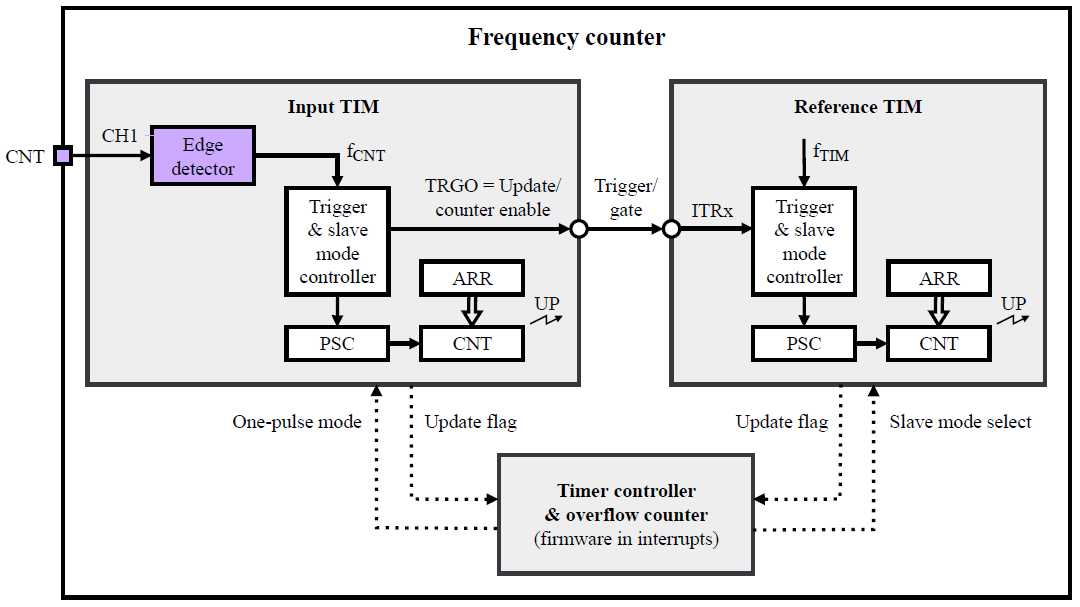
\includegraphics[width=0.7\linewidth]{Figs/Documentation/DujavaFrequencyCounter}
 	\caption{Diagram propojení čítačů pro upravenou metodu měření frekvence čítáním pulzů. Převzato z \cite{DujavaDIP}}
 	\label{fig:dujavafrequencycounter}
 \end{figure}
 
 Časový diagram měření je znázorněn na obrázku \ref{fig:PulseCounter} s tím, že TIMx označuje vstupní čítač a TIMy čítač referenční. Průběh měření se dá popsat následujícími kroky:
 \begin{itemize}
 	\item Měření je zahájeno zapnutím vstupního čítače. TIMx\_CEN = 1;
 	\item První nástupní hrana vstupního signálu vyresetuje oba čítače a zapne referenční čítač, který začne odměřovat uběhlý čas pomocí interních hodin PCLK.
 	\item Po uplynutí stanovené doby $t_{\text{gate}}$ se nastaví kolik $n$ vstupních period signálu se ještě má odměřit pro doběhnutí měření. Toho docílíme nastavením registru ARR vstupního čítače na aktuální hodnotu CNT registru zvýšenou o $n$ a nastavením vstupního čítače do One pulse režimu (OPM).
 	\item Díky nastavenému OPM režimu se po doběhnutí vstupního čítače do hodnoty ARR oba čítače automaticky zastaví.
 \end{itemize}
 
 
 
 \begin{figure}[H]
 	\centering
 	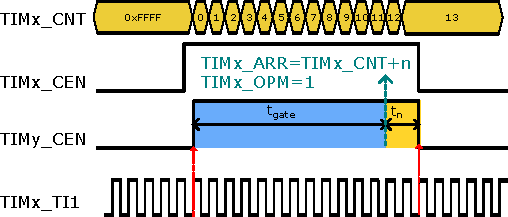
\includegraphics[width=0.7\linewidth]{Figs/Diagrams/SVG/PulseCounter.pdf}
 	\caption{Časový diagram čítání pulzů za proměnnou dobu odběru}
 	\label{fig:PulseCounter}
 \end{figure}
 
 Výše popsaným způsobem získáme dobu měření $T_{\text{meas}}=t_{\text{gate}}+ t_{\text{n}}$ a počet period vstupního signálu $N$, které se za tu dobu objevily na vstupu. Čas měření jsme schopní měřit v rozlišení daném frekvencí interních hodin čítače. V mém případě $f_{\text{TIM}}=156 \text{ MHz} $, což znamená že dobu měření stovujeme v krocích asi 6.4 ns. Výslednou frekvenci vstupního signálu $f_{\text{in}}$, pak získáme tímto přepočtem:
 
 \begin{equation}
 	f_{\text{in}}=\frac{N}{T_{\text{meas}}}
 \end{equation}
 
